\documentclass[12pt]{article}
\usepackage{hyperref}
\usepackage{amsmath}
%\usepackage{amsmath}
\usepackage{graphicx}
\usepackage{xspace}
% \usepackage[extendedchars]{grffile}
\usepackage{chngpage}
\usepackage{calc}
\usepackage{topcapt}
\newcommand{\unit}[1]{\ensuremath{\text{\,#1}}\xspace}
\newcommand{\fbinv} {\mbox{\ensuremath{\,\text{fb}^{-1}}}\xspace}
\newcommand{\pbinv} {\mbox{\ensuremath{\,\text{pb}^{-1}}}\xspace}


\title{Analysis of the milliQan demonstrator data at the LHC}

\author{M. Citron}

\begin{document}
\maketitle

\section{Introduction}

The collection, calibration and analysis of the milliqan demonstrator data is described below.

\section{The milliQan demonstrator}

Details of the milliQan demonstrator. The channel mapping is shown in Figure~\ref{fig:channelMap}.

\begin{figure}
\centering
    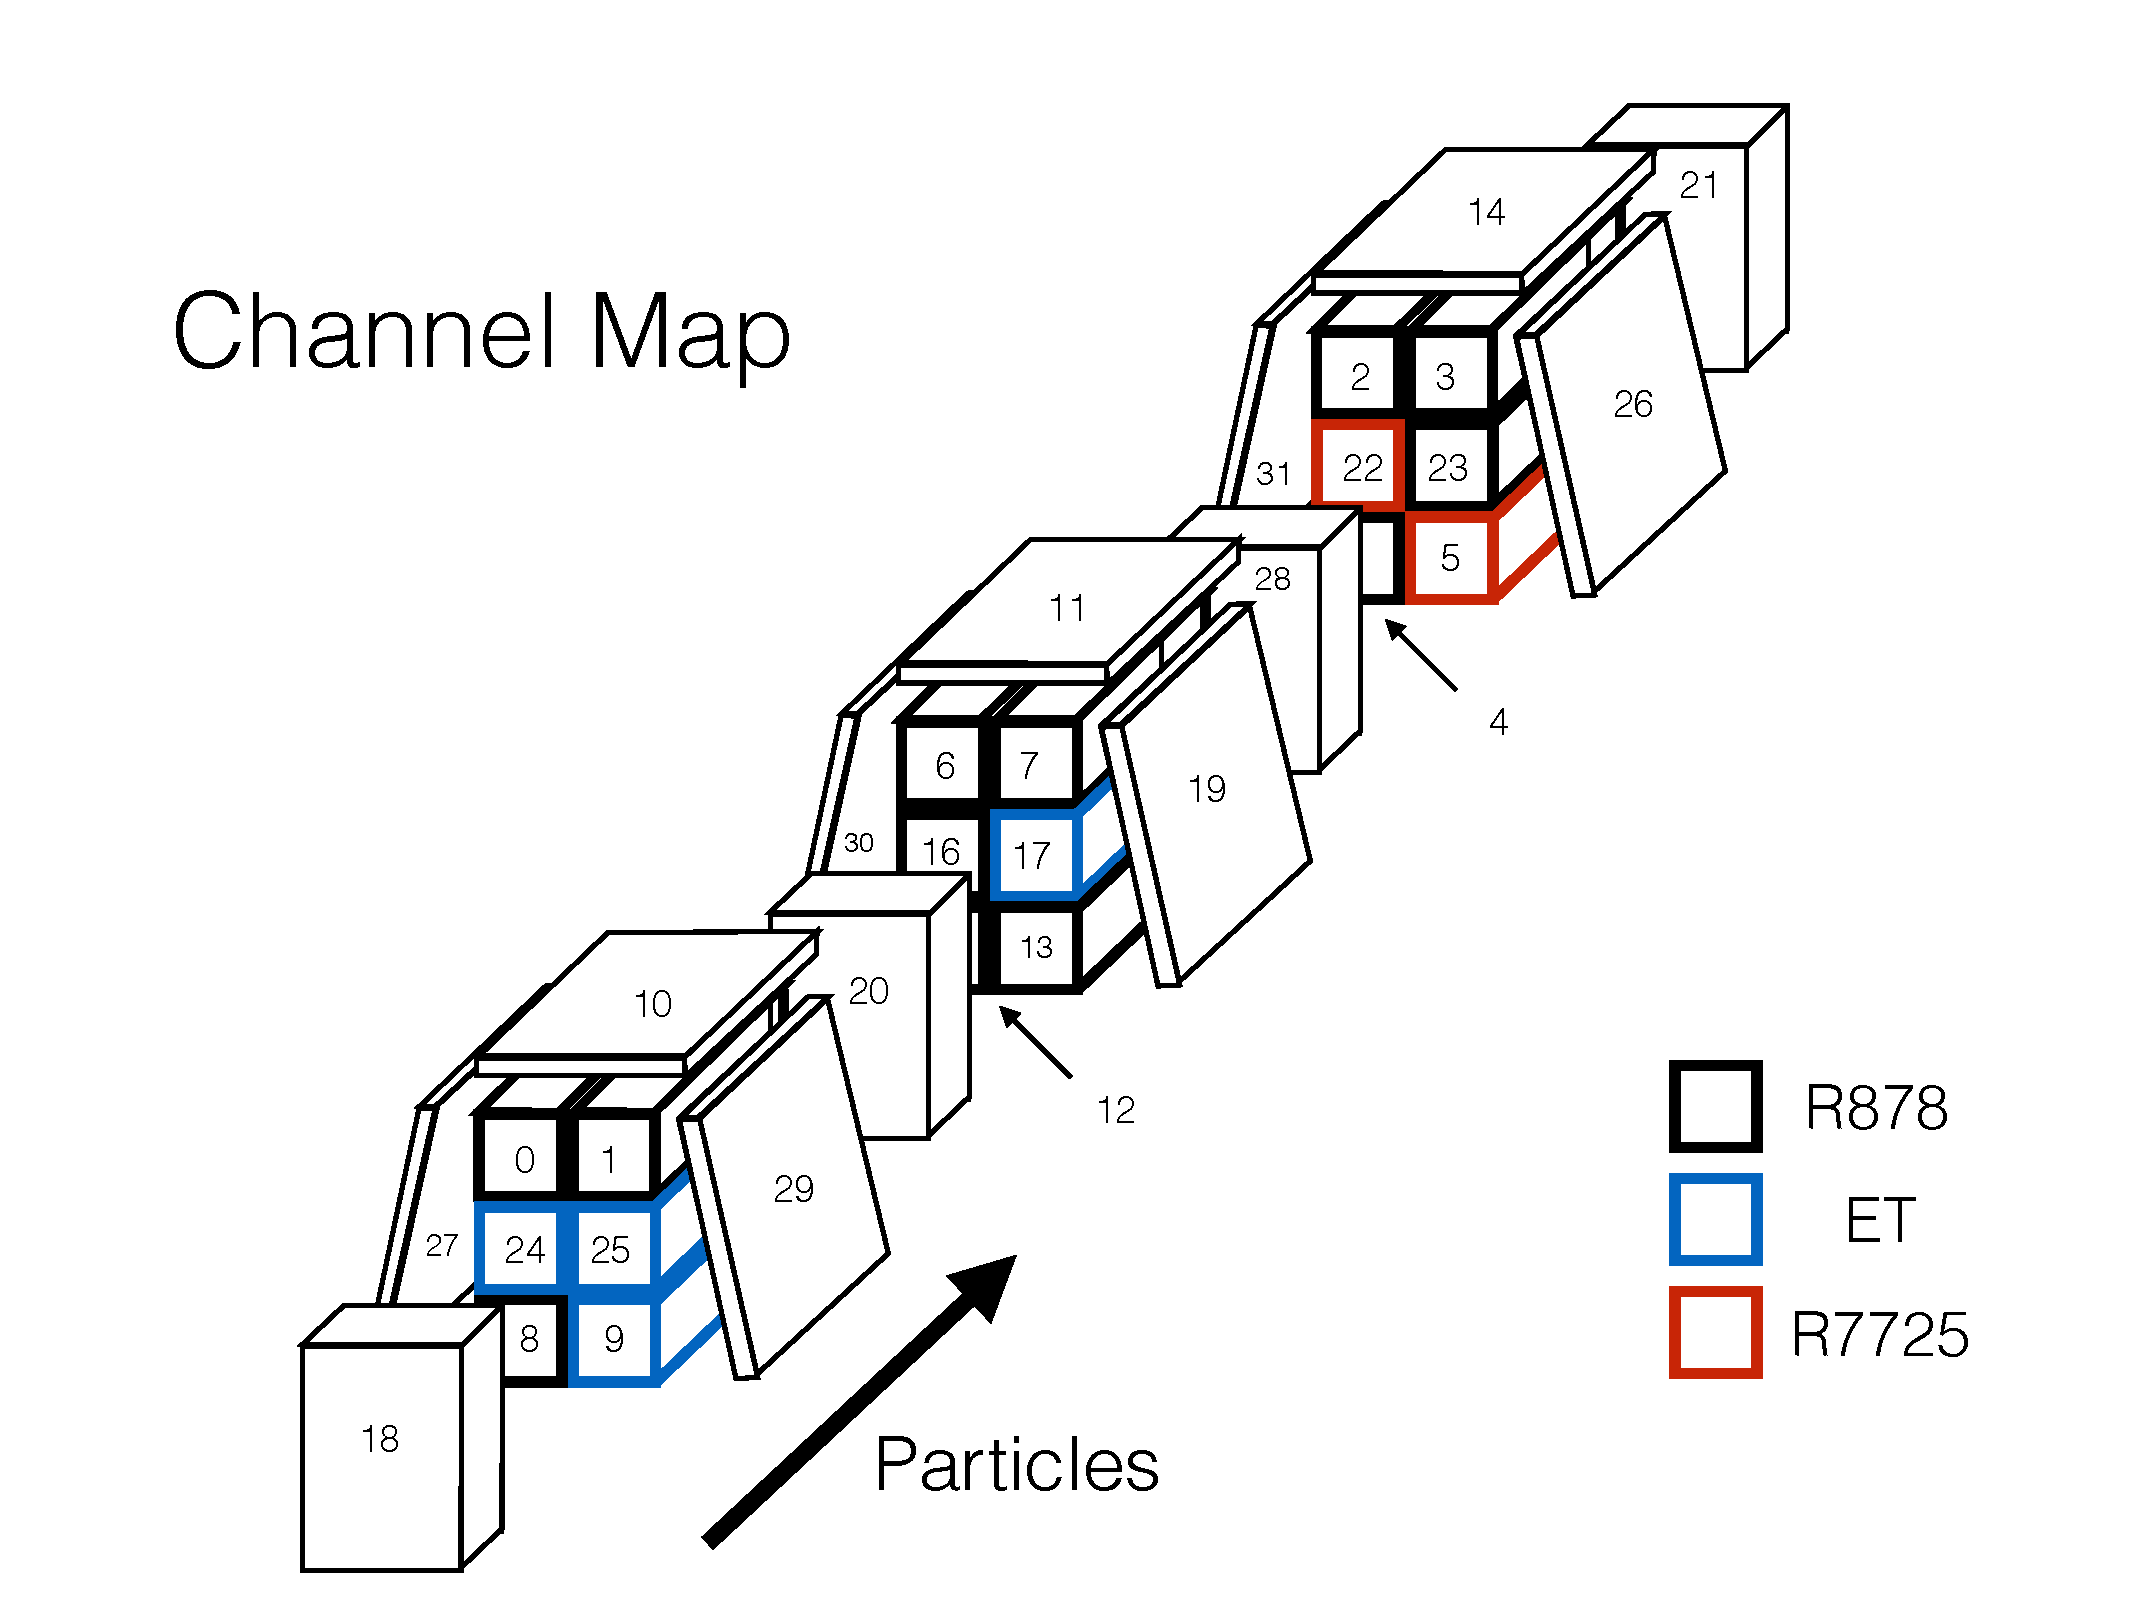
\includegraphics[width=0.6\textwidth]{figures/channelMap}
    \caption{\label{fig:channelMap} The channel mapping for the milliQan demonstrator. 
    The PMT species are indicated by the colour.}
\end{figure}

\section{Data taking}

The data considered in this analysis was collected by the milliQan demonstrator between June 26th 2018 and October 21st 2018.
For all physics quality data, the PMT high voltage is set to $1300\unit{V}$ for the R7725s, $1450\unit{V}$ for the R878s
and $1550\unit{V}$ for the Electron Tubes (ETs). Events are triggered if there is a signal above the trigger threshold 
in three trigger groups within a window of $100\unit{ns}$. Each trigger group contains two channels and the trigger
group for each channel is given by floor(channel/2). The channel mapping ensures adjacent bars are in the same trigger group. 

The trigger thresholds varied during data taking to satisfy rate requirements. The typical 
threshold for the bars ranges from $2.4--7\unit{mV}$, the typical value for the slabs ranges from $150-400\unit{mV}$ and 
for the panels ranges from $2.5--40\unit{mV}$.
%FIXME Add correct values for all years (info needed in tree!)

The total data taking time of all physics runs is $2014.6\unit{h}$. When the data taking rate is high
events may not be properly synched between the two digitiser boards used for reading channels 0-15 and 
channels 16-32. To reject unsynched events, a requirement is made that both boards record
the TDC time. The efficiency of this selection is $\sim 95\%$ giving an effective total
time of $1906.4\unit{h}$, with approximately $876.9\unit{h}$ and $1029.5\unit{h}$ 
taken during between periods with and without LHC proton-proton collisions respectively.
The total proton-proton luminosity collected is $37.2\fbinv$, of which $35.1\fbinv$ 
satisfies the synchronisation requirement. 

\begin{table}[ht!]
    \scriptsize
    \centering
    \topcaption{
	Mean and RMS for each channel measured in the sideband region of a physics run \label{tab:sideband}
    }
    \begin{tabular}{lll}
	Channel & Sideband mean (mV)& Sideband RMS (mV)\\
	\hline
	    0 & -0.2453  & 0.8637    \\      
	    1 &  0.009&     0.7901   \\
	    2 &  -0.007  &  0.9028   \\ 
	    3 &  -0.07&     0.7561   \\
	    4 &  -0.661&    0.8741   \\
	    5 &  -0.252&    0.7857   \\
	    6 &  0.080&     0.8706   \\
	    7 &  -0.214&    0.7795   \\
	    8 &  -1.04&     0.8098   \\
	    9 &  -0.160&    0.7954   \\
	    10 & 1.18&      0.9941   \\
	    11 & -0.910&    0.7833   \\
	    12 & -0.3789 &  0.9148   \\  
	    13 & -1.09&     0.7899   \\
	    14 & -0.53&     0.9600   \\
	    15 & --&        --       \\
	    16 & -0.367&    0.8829   \\
	    17 & -0.837&    0.8828   \\
	    18 & -0.283&    0.8908   \\
	    19 & -0.275&    0.8005   \\
	    20 & -0.235&    0.8400   \\
	    21 & -0.295&    0.8863   \\
	    22 & -0.443&    1.061    \\
	    23 & -0.606&    0.8085   \\
	    24 & -0.762&    0.9275   \\
	    25 & -0.201&    0.8194   \\
	    26 & -0.576&    0.9087   \\
	    27 & -0.440&    0.7757   \\
	    28 & -0.706&    0.8507   \\
	    29 & -0.426&    0.9169   \\
	    30 & -0.280&    0.9577   \\
	    31 & -0.458  &  0.8018   \\ 
    \end{tabular}
\end{table}
\section{Reconstruction}

The data taken by the demonstrator is comprised of "waveforms" of voltage against time for each channel.
In order to reconstruct the deposits of particles in the scintillator, "pulses" are reconstructed from
each waveform. 

With a sampling rate of 1.6 Ghz, the waveforms span $0$ to $XX\unit{ns}$ (with the pulse
that causes the trigger to accept the event placed at $\sim360 -- 390 \unit{ns}$).
The waveforms may have a significant pedestal which is measured using the mean
value of the amplitude in a sideband region of the waveform from $0 -- 50 \unit{ns}$.
The mean value of this pedestal measurement for each channel in a physics run 
is used to define a pedestal subtraction with the values
shown in Table~\ref{tab:sideband}. Significant drifts are seen in the pedestal for channel 30
and so a subtraction is made using the sideband pedestral measurement per event.

After the pedestral subtraction pulses are reconstructed from the waveforms. Starting from the first sample after the sideband region, 
the algorithm runs considers each time sample consecutively and runs as follows until a pulse is started:

\begin{itemize}
    \item If the sample is above the start threshold in Table~\ref{tab:pulseFinding}, increment the pulse starting counter.
    \item If the sample is below the reset threshold in Table~\ref{tab:pulseFinding}, reset the pulse starting counter. This threshold is set as the start threshold minus half the sideband RMS shown in Table~\ref{tab:sideband}.
    \item if the pulse starting counter reaches the N samples above start threshold value shown in Table~\ref{tab:pulseFinding}, start a pulse.
\end{itemize}

Once a pulse has been started the pulse end is determined by continuing as follows:

\begin{itemize}
    \item If the sample is below the start threshold in Table~\ref{tab:pulseFinding}, increment the pulse ending counter. 
    \item If the sample is above the reset pulse end threshold in Table~\ref{tab:pulseFinding} reset the pulse ending counter. This threshold is set as the start threshold plus half the sideband RMS shown in Table~\ref{tab:sideband}.
    \item if the pulse ending counter reaches the N samples below start threshold value shown in Table~\ref{tab:pulseFinding}, end the pulse.
\end{itemize}

Each pulse has several attributes defined as follows:

\begin{description}
    \item[time] The time of the last sample below the start threshold before the pulse is started.
    \item[calibrated time] The calibrated time of the pulse as defined in Section~\ref{sec:timeCalibration}.
    \item[duration] The time of the sample after that which triggers the pulse ending minus the time of the last sample below the start threshold.
    \item[height] The maximum amplitude in the pulse.
    \item[area] The sum of the amplitudes across the pulse.
    \item[nPE] The area divided by the SPE area for each channel (measured as described in Section~\ref{sec:npeCalibration}).
    \item[delay] Time between start of this pulse and end of previous pulse.
\end{description}

\begin{table}[ht!]
    \scriptsize
    \centering
    \topcaption{
	Pulse finding thresholds. \label{tab:pulseFinding}
    }
    \begin{tabular}{lllll}
	N samples above & N samples below& Start threshold (mV) & Reset threshold (mV) & End threshold (mV)\\
	start threshold & end threshold &  &  & \\
	\hline
	7 & 13 & 2.0 & 1.57 & 2.43\\
	7 & 13 & 2.0 & 1.60 & 2.40\\
	9 & 13 & 2.3 & 1.85 & 2.75\\
	7 & 13 & 2.0 & 1.62 & 2.38\\
	7 & 13 & 2.2 & 1.76 & 2.64\\
	5 & 4 & 2.0 & 1.61 & 2.39\\
	7 & 13 & 2.0 & 1.56 & 2.44\\
	7 & 13 & 2.0 & 1.61 & 2.39\\
	7 & 13 & 2.0 & 1.60 & 2.40\\
	4 & 4 & 2.0 & 1.60 & 2.40\\
	7 & 13 & 2.2 & 1.70 & 2.70\\
	7 & 13 & 2.0 & 1.61 & 2.39\\
	7 & 13 & 2.0 & 1.54 & 2.46\\
	8 & 13 & 2.0 & 1.61 & 2.39\\
	9 & 13 & 2.3 & 1.82 & 2.78\\
	7 & 13 & 2.5 & 2.00 & 3.00\\
	7 & 13 & 2.0 & 1.56 & 2.44\\
	4 & 4 & 2.0 & 1.56 & 2.44\\
	8 & 13 & 2.0 & 1.55 & 2.45\\
	7 & 13 & 2.0 & 1.60 & 2.40\\
	7 & 13 & 2.0 & 1.58 & 2.42\\
	8 & 13 & 2.0 & 1.56 & 2.44\\
	5 & 4 & 3.7 & 3.17 & 4.23\\
	7 & 13 & 2.0 & 1.60 & 2.40\\
	4 & 4 & 2.0 & 1.54 & 2.46\\
	4 & 4 & 2.0 & 1.59 & 2.41\\
	7 & 13 & 2.0 & 1.55 & 2.45\\
	7 & 13 & 2.0 & 1.61 & 2.39\\
	7 & 13 & 2.0 & 1.57 & 2.43\\
	7 & 13 & 2.0 & 1.54 & 2.46\\
	7 & 13 & 2.0 & 1.52 & 2.48\\
	7 & 13 & 2.0 & 1.60 & 2.40\\
    \end{tabular}
\end{table}

\section{Calibration}

\subsection{NPE calibration}
\label{sec:npeCalibration}
Calibration of the SPE area and NPE.

\subsection{Time calibration}
\label{sec:timeCalibration}

The timing calibration is crucial to achieve the targeted $\sim15\unit{ns}$ window between pulses arriving in each layer
in order to effectively reject backgrounds from uncorrelated sources. The calibration
procedure is designed such that a muon travelling upwards through the detector 
from the beam should have the same time
value in every channel.

First, channels in the same "slice" (left or right side of each layer) are calibrated 
using down-going cosmic muons, tagged as a muon pulse hitting the top panel and 
each channel in a particular slice. The mean value of the time difference of each channel relative to the top channel of each slice 
is taken as the calibration. Figure~\ref{fig:timeDiffIntraSlice} shows the time difference between the channels for several example calibrations.
The standard deviation ranges from 1.7 to 2.8\unit{ns}.

\begin{figure}
\centering
    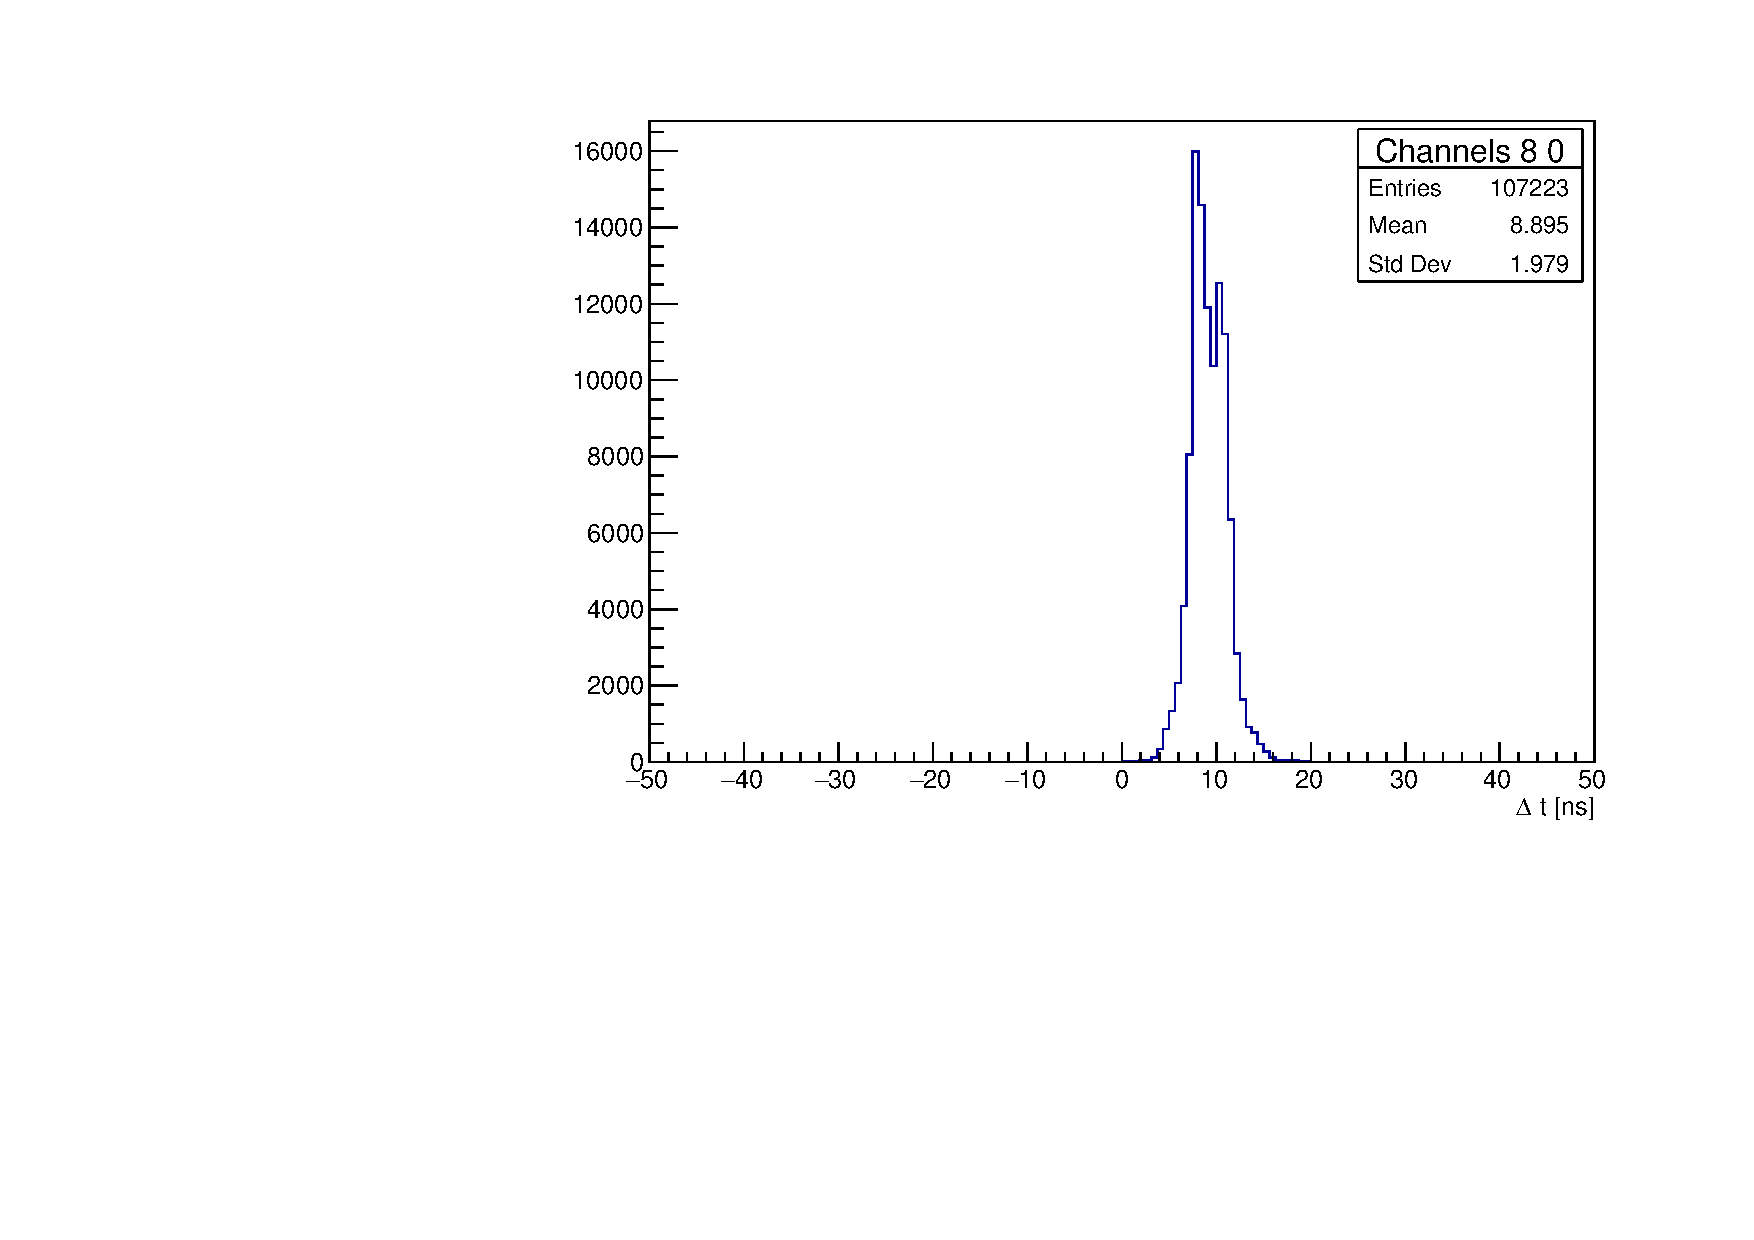
\includegraphics[width=0.49\textwidth]{figures/timingPlots/intraSlice/Channels_8_0.pdf}~
    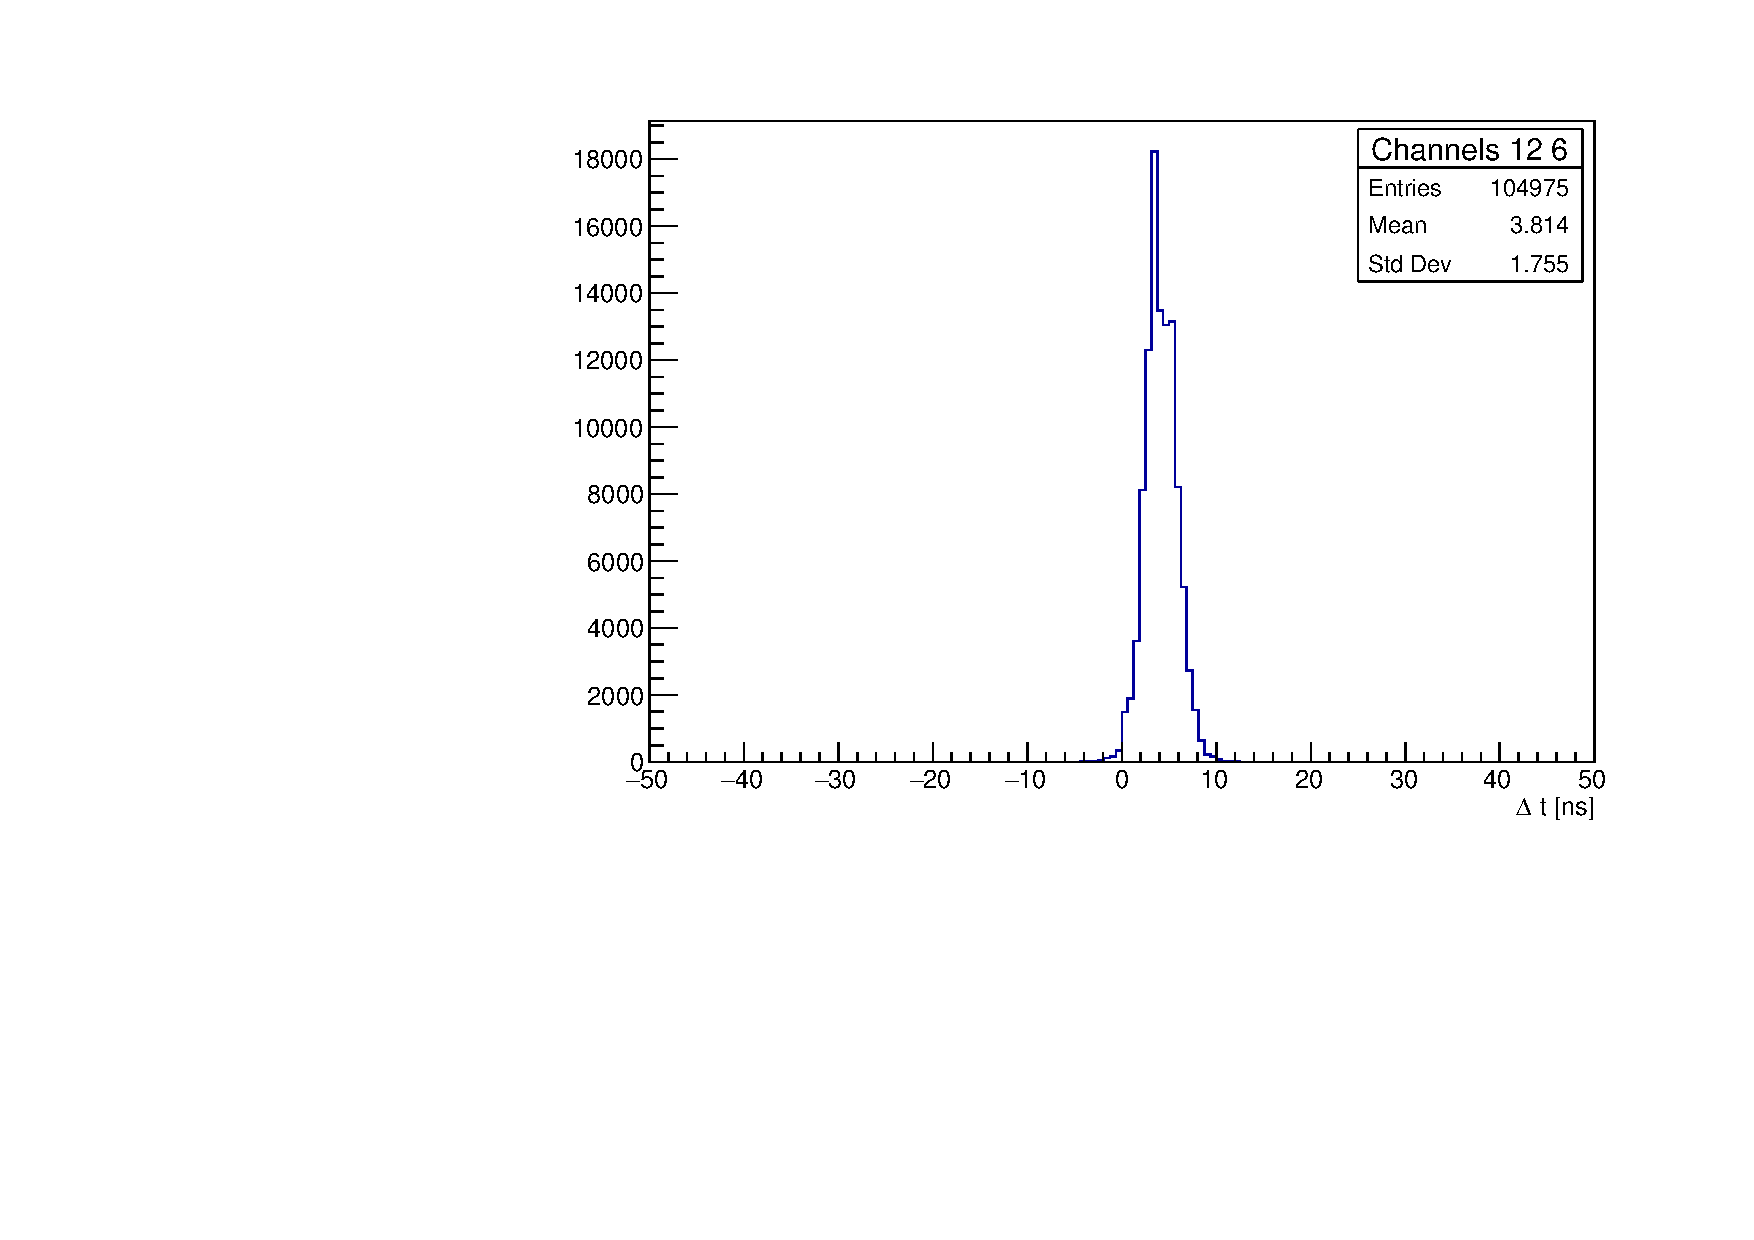
\includegraphics[width=0.49\textwidth]{figures/timingPlots/intraSlice/Channels_12_6.pdf}\\
    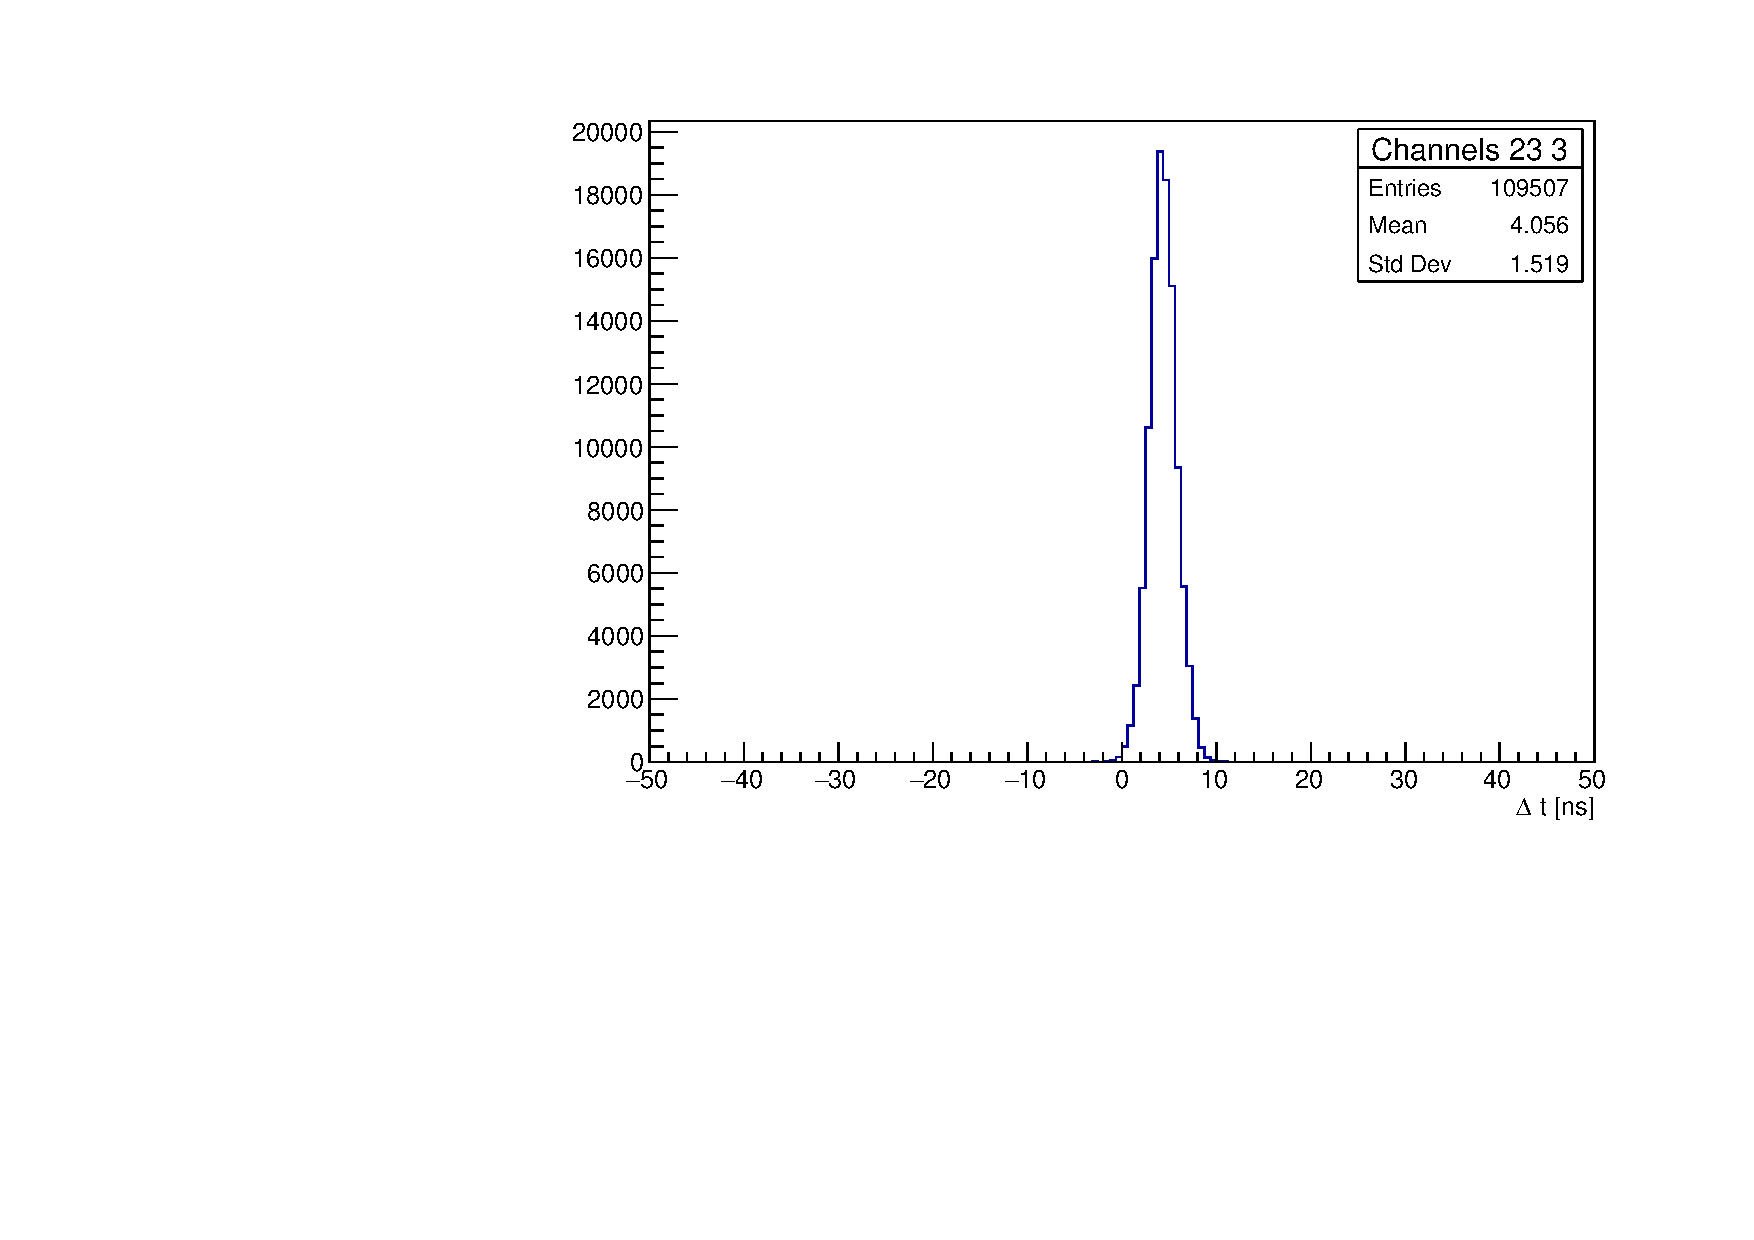
\includegraphics[width=0.49\textwidth]{figures/timingPlots/intraSlice/Channels_23_3.pdf}~
    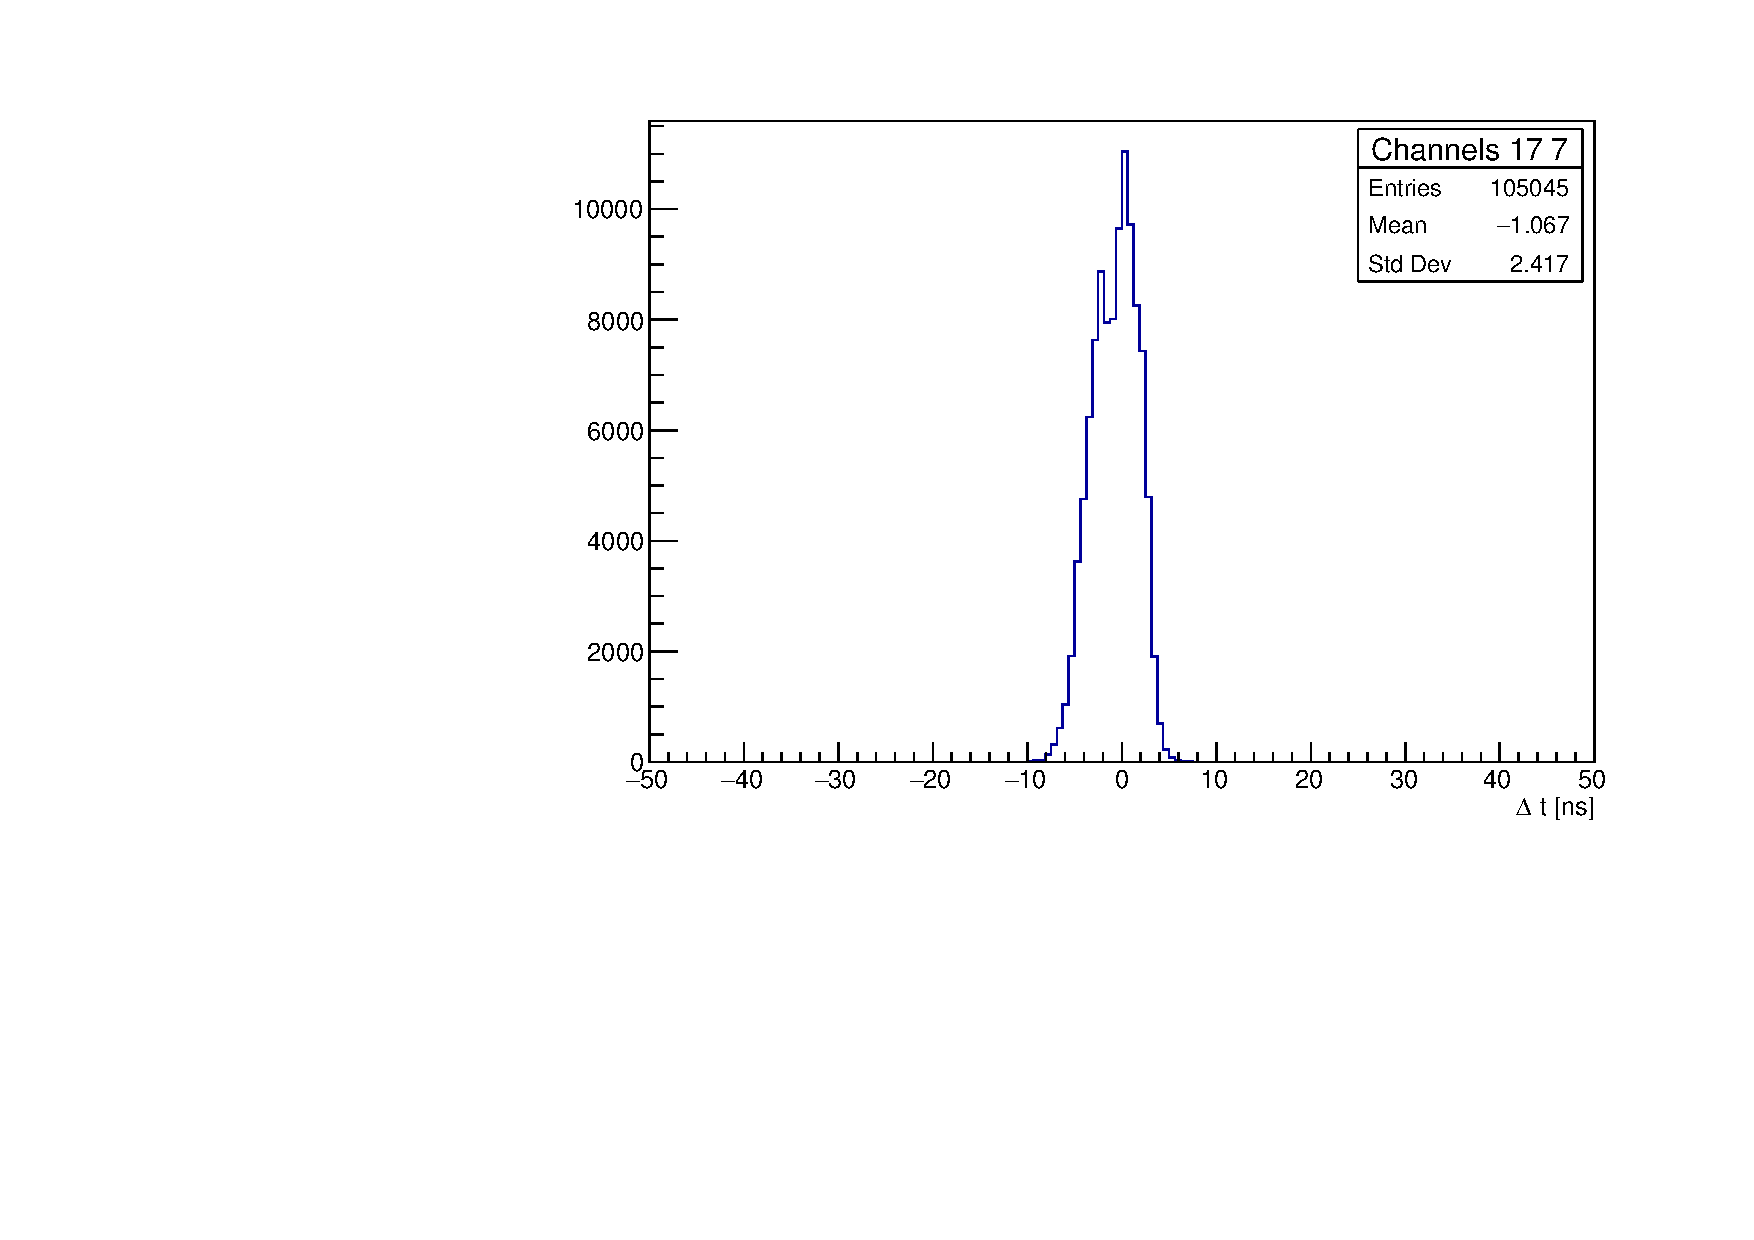
\includegraphics[width=0.49\textwidth]{figures/timingPlots/intraSlice/Channels_17_7.pdf}
    \caption{\label{fig:timeDiffIntraSlice} Example time differences between channels in the same slices. The mean values are used to calibrate the intra-slice timing.}
\end{figure}

After applying the intra-slice calibration, the slices are then calibrated using down-going cosmic muons, tagged as muon pulse hitting the top panel and both slices in a particular layer.
The mean value of the time difference relative to the left slice of each layer is taken as the calibration.
Figure~\ref{fig:timeDiffIntraLayer} shows the time difference between the slices for each layer.
The standard deviation ranges from 2.3 to 2.8\unit{ns}.

\begin{figure}
\centering
    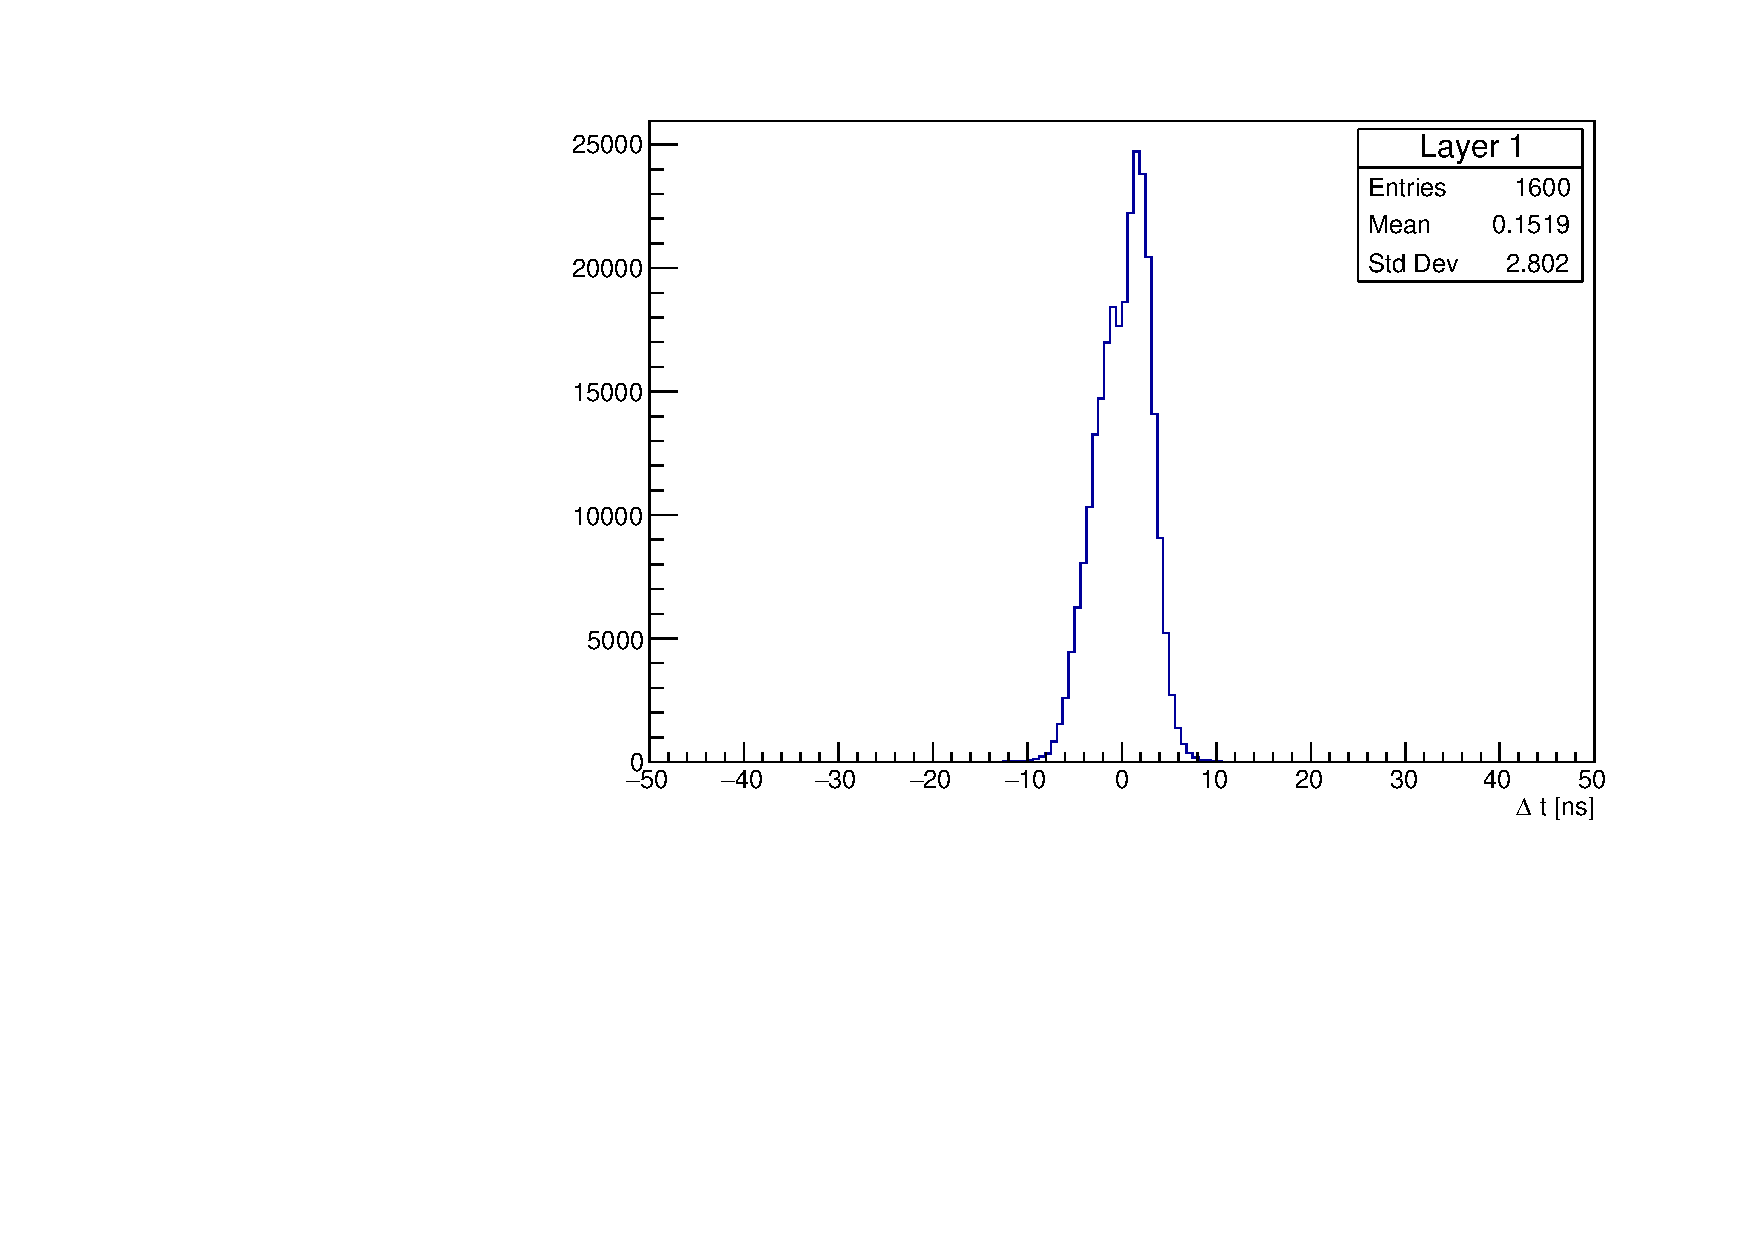
\includegraphics[width=0.49\textwidth]{figures/timingPlots/intraLayer/Layer_1.pdf}~
    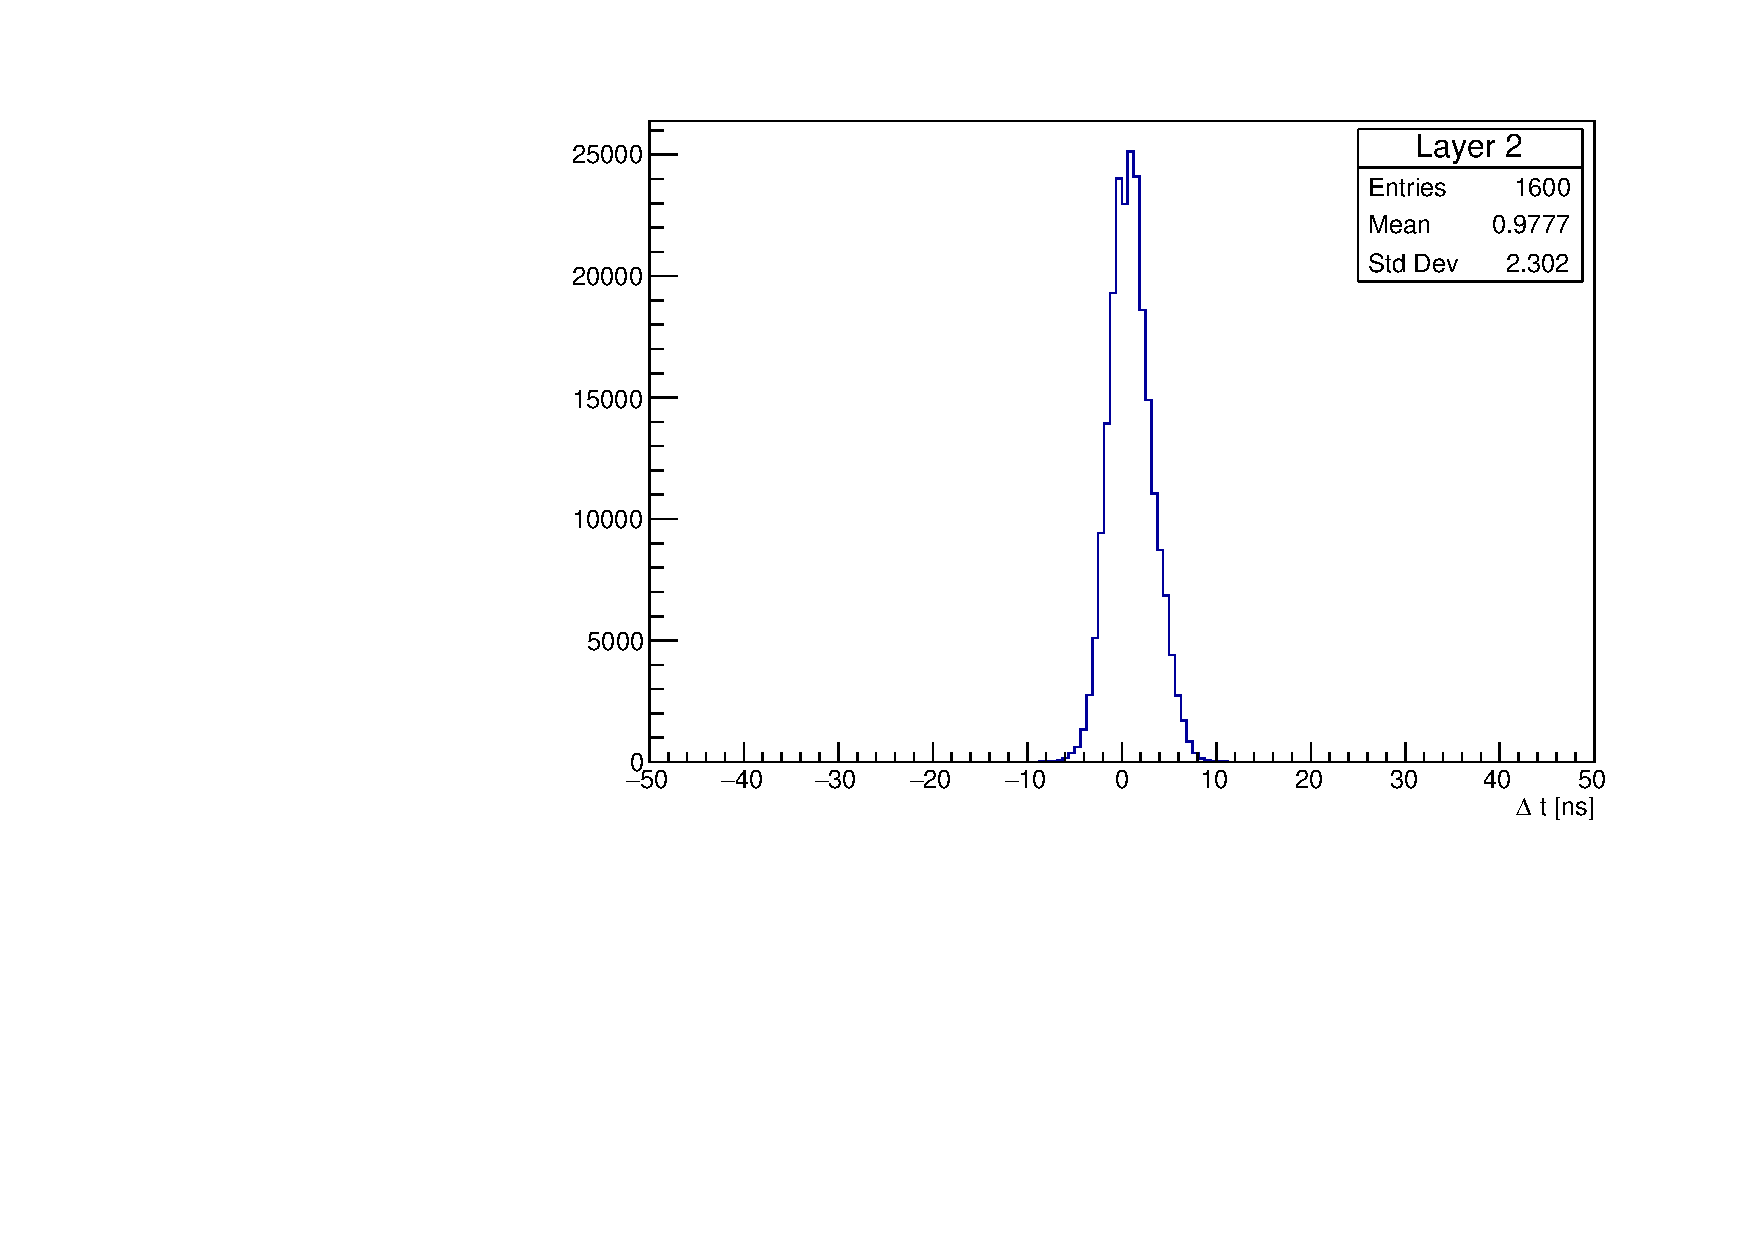
\includegraphics[width=0.49\textwidth]{figures/timingPlots/intraLayer/Layer_2.pdf}\\
    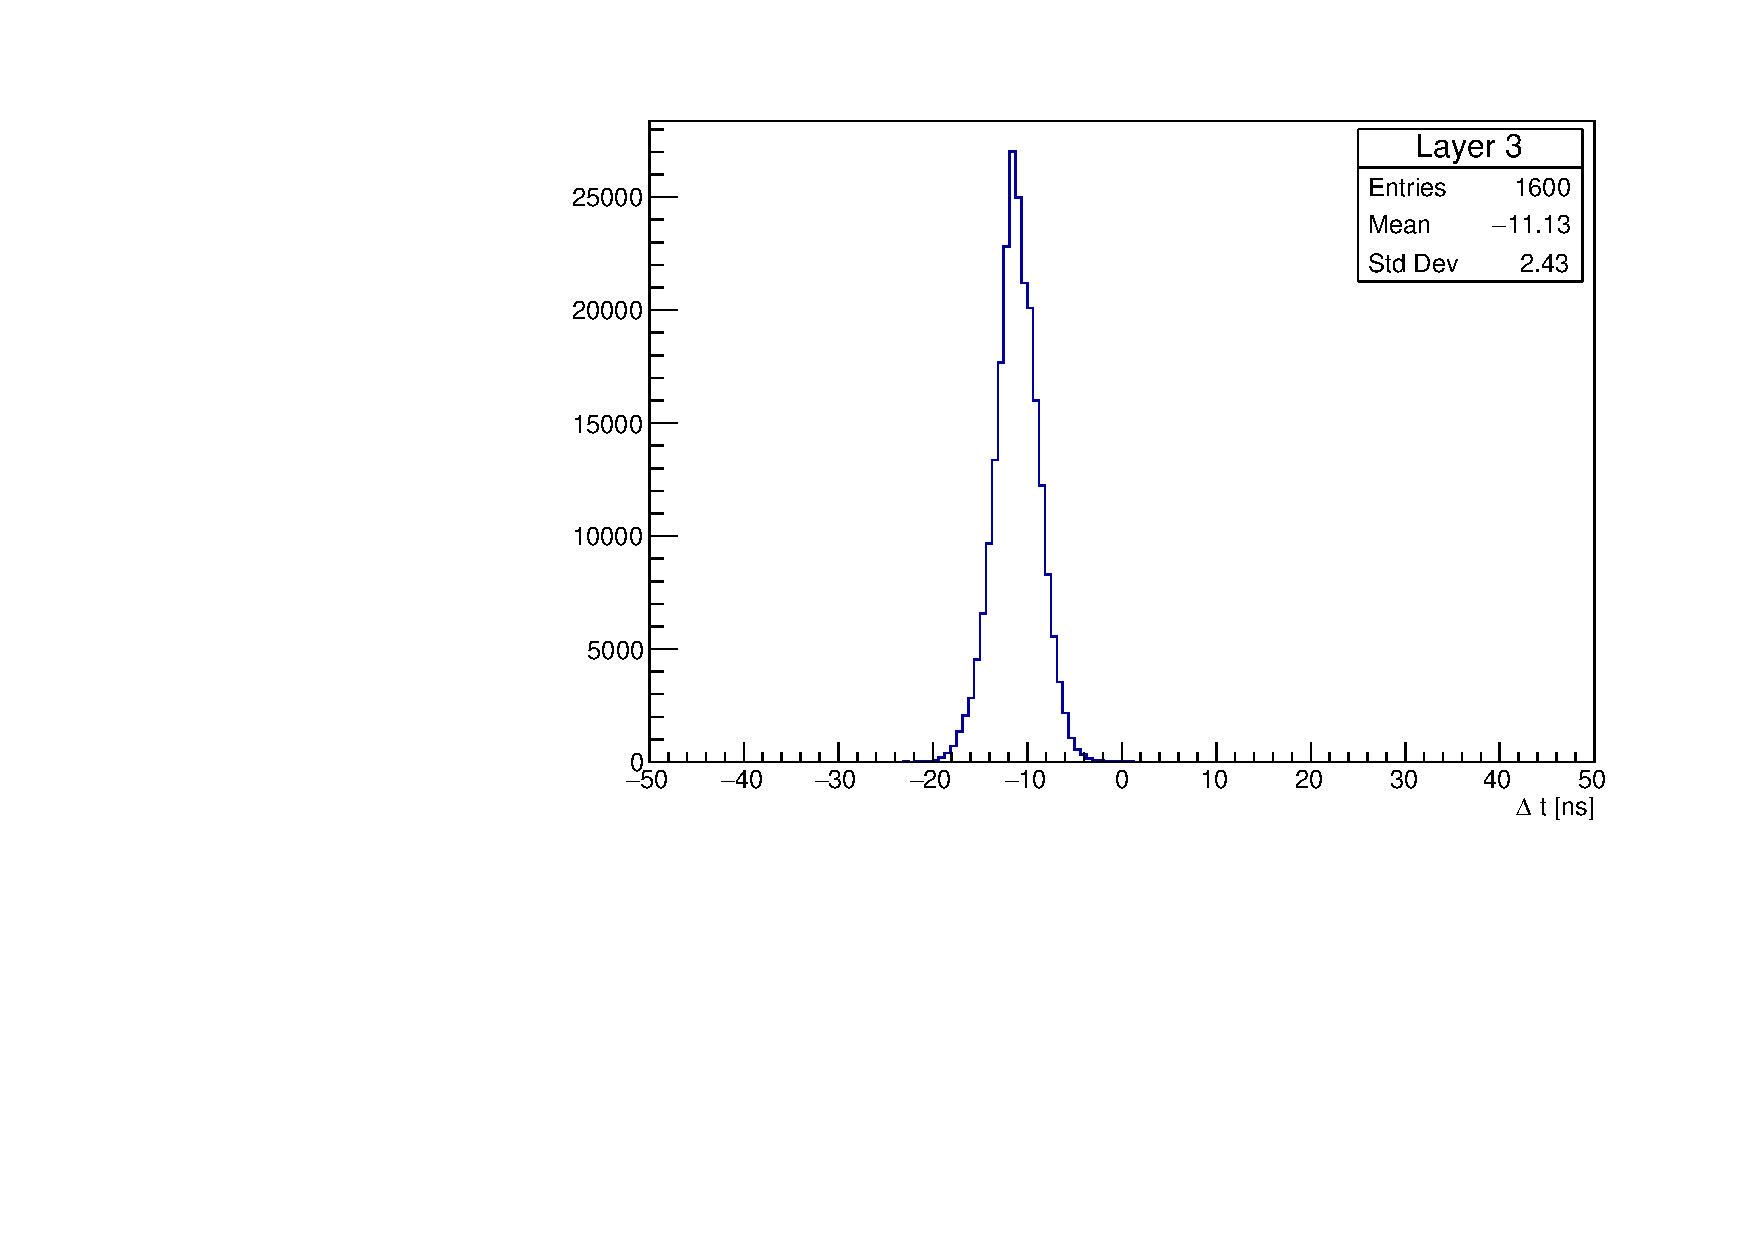
\includegraphics[width=0.49\textwidth]{figures/timingPlots/intraLayer/Layer_3.pdf}
    \caption{\label{fig:timeDiffIntraLayer} Time differences between slices in the same layer for all layers. The mean values are used to calibrate the intra-layer timing.}
\end{figure}

The slab timing is then calibrated using beam muons, tagged as a muon pulse 
hitting all four slabs. In order to avoid bias from cosmic muons, the modal 
value of the time difference relative to the slab closest to the CMS IP (channel 18) 
is taken as the calibration. Figure~\ref{fig:timeDiffInterSlab} shows
the time difference between the slabs and channel 18. 

\begin{figure}
\centering
    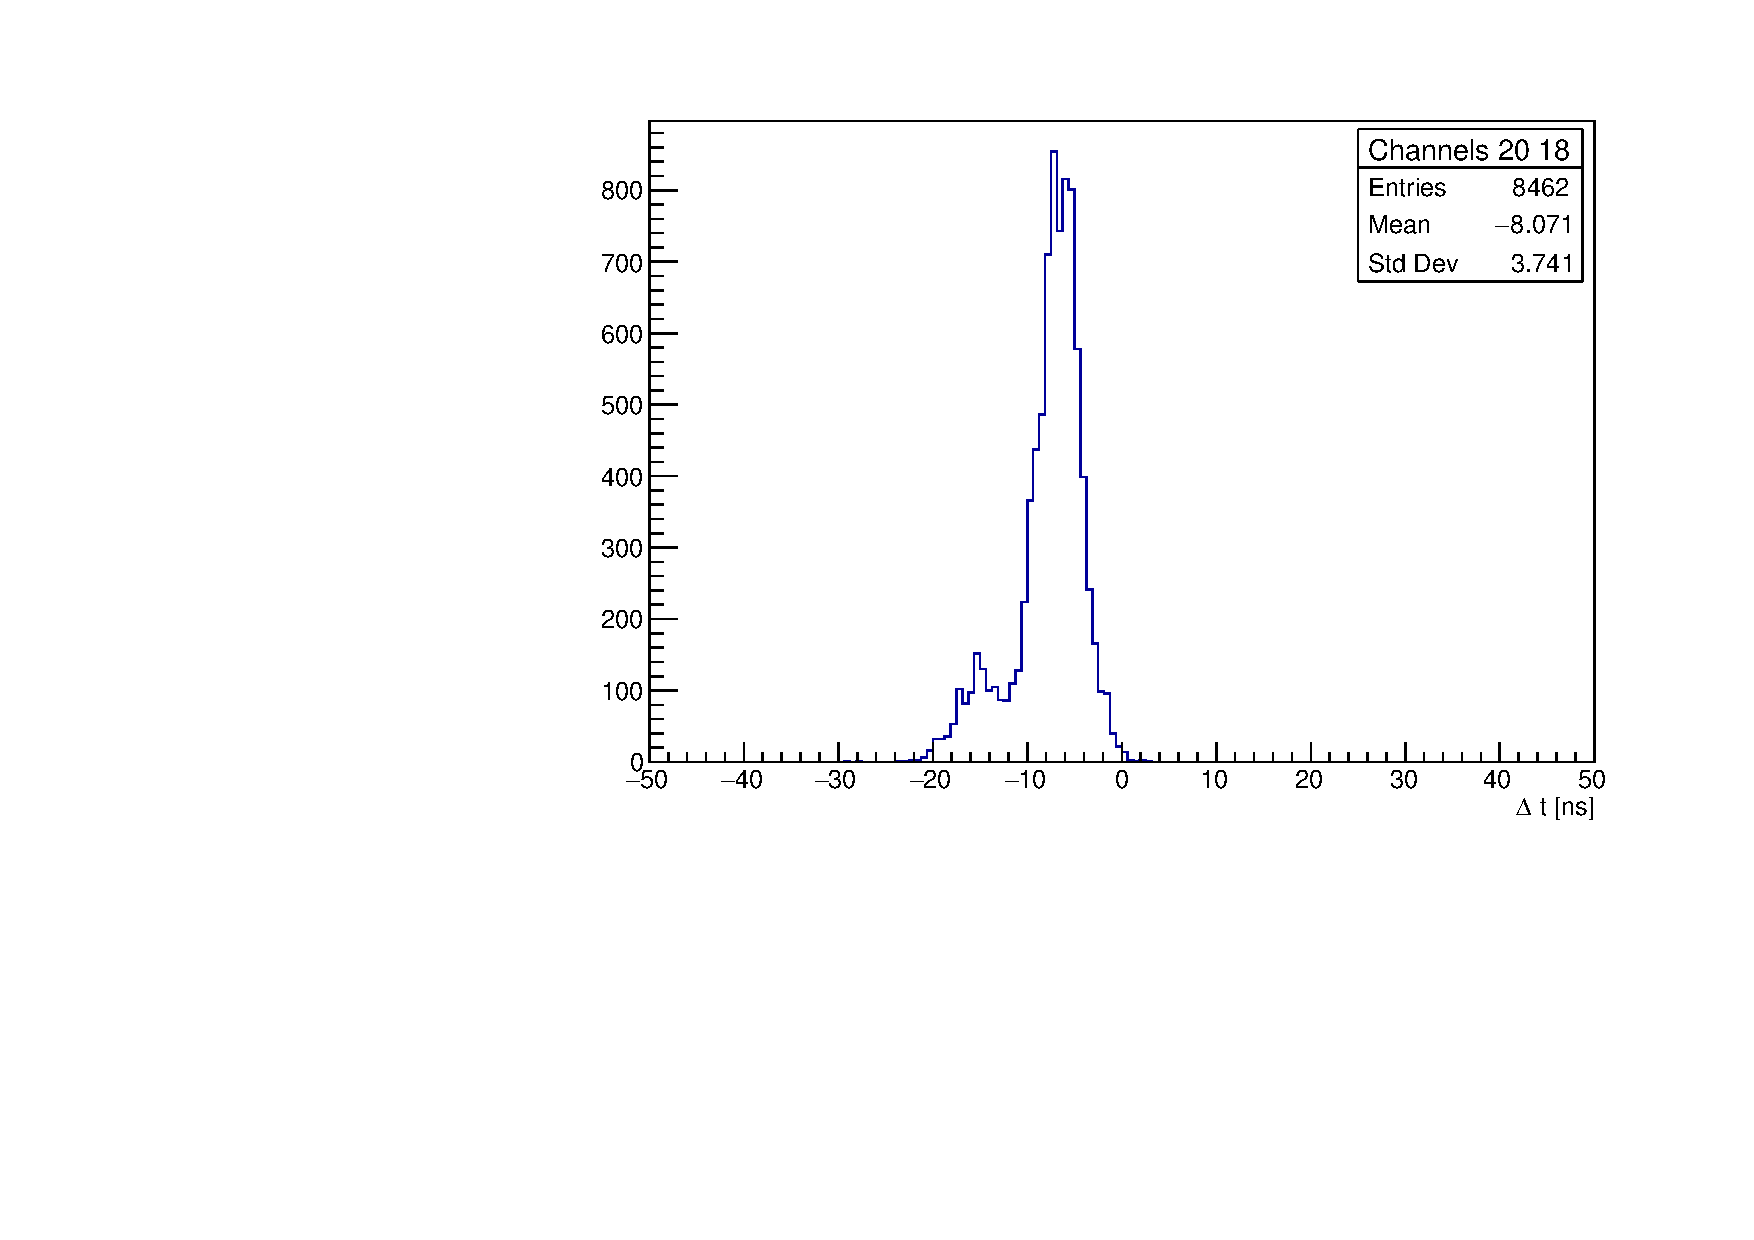
\includegraphics[width=0.49\textwidth]{figures/timingPlots/intraSlice/Channels_20_18.pdf}~
    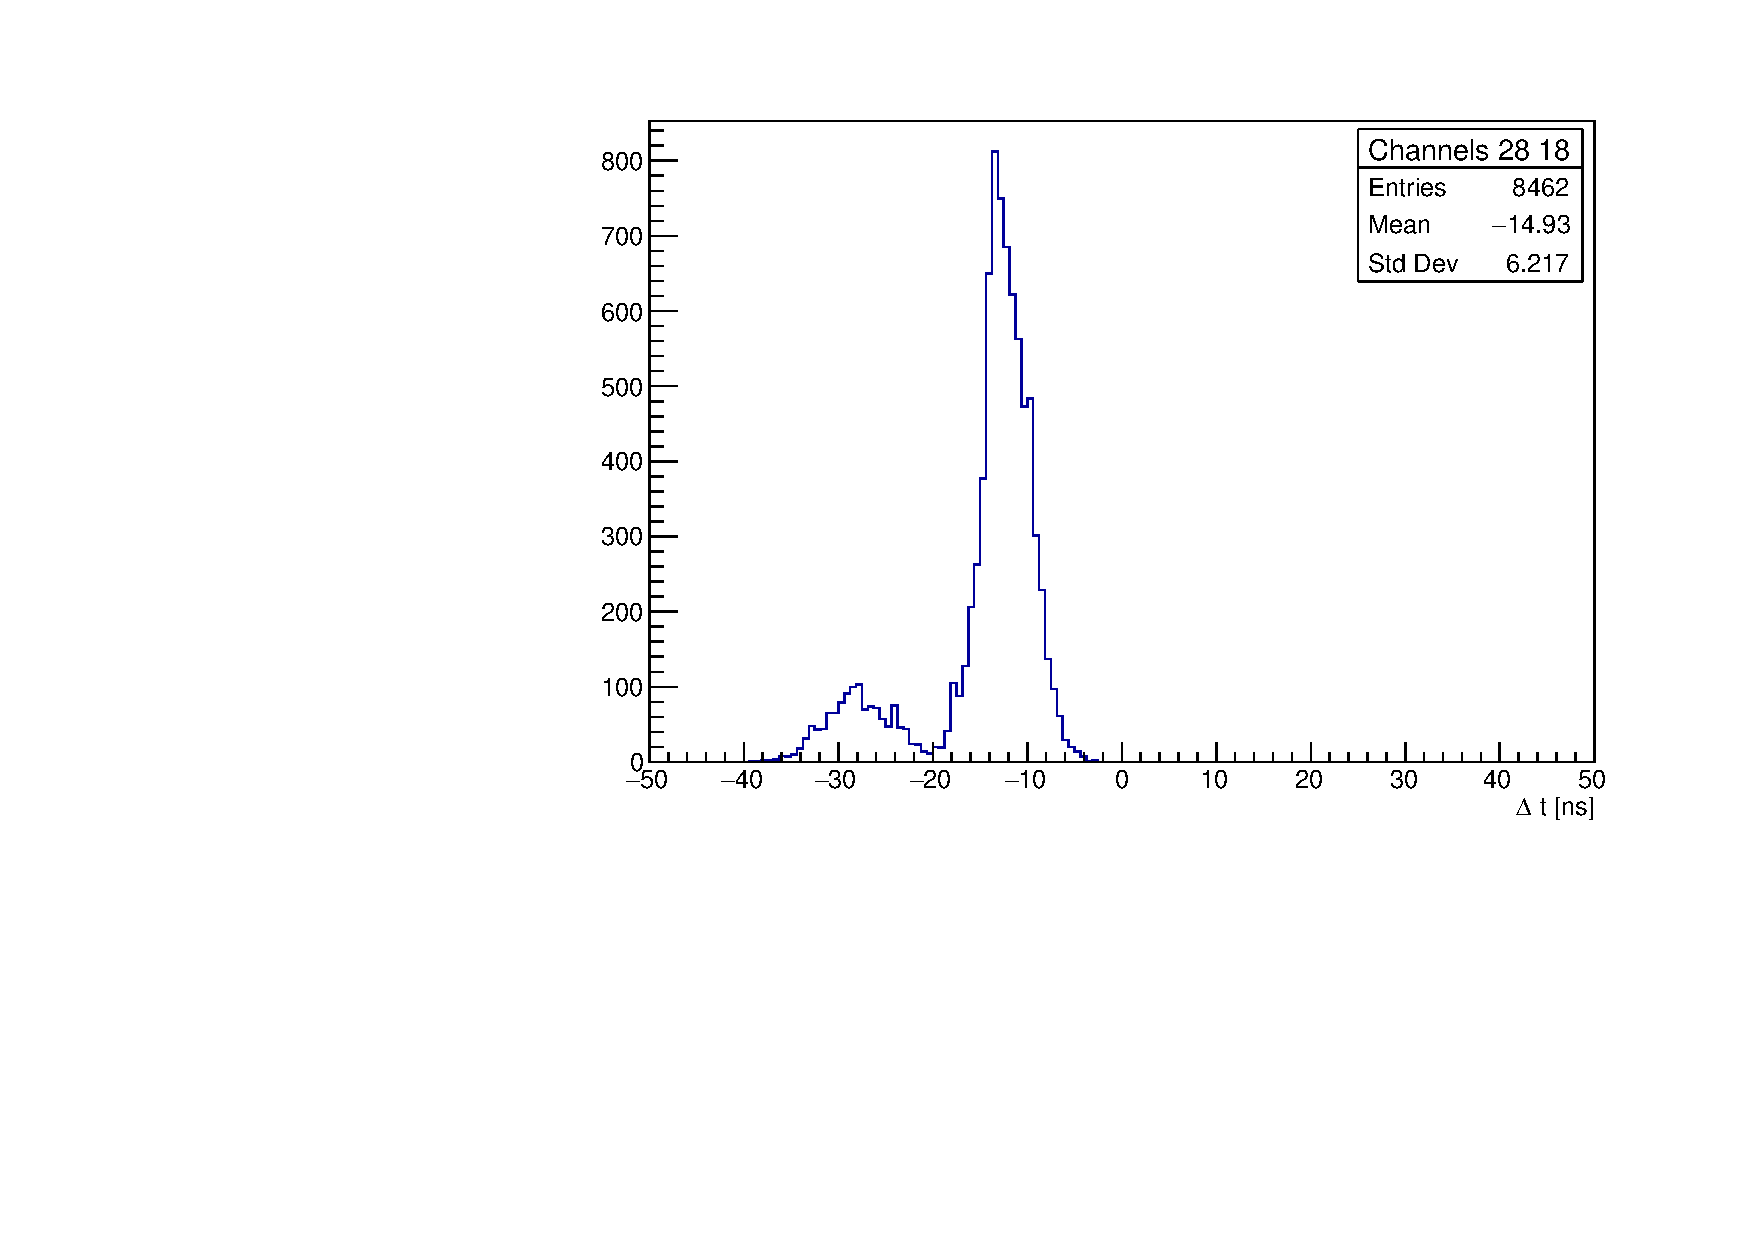
\includegraphics[width=0.49\textwidth]{figures/timingPlots/intraSlice/Channels_28_18.pdf}\\
    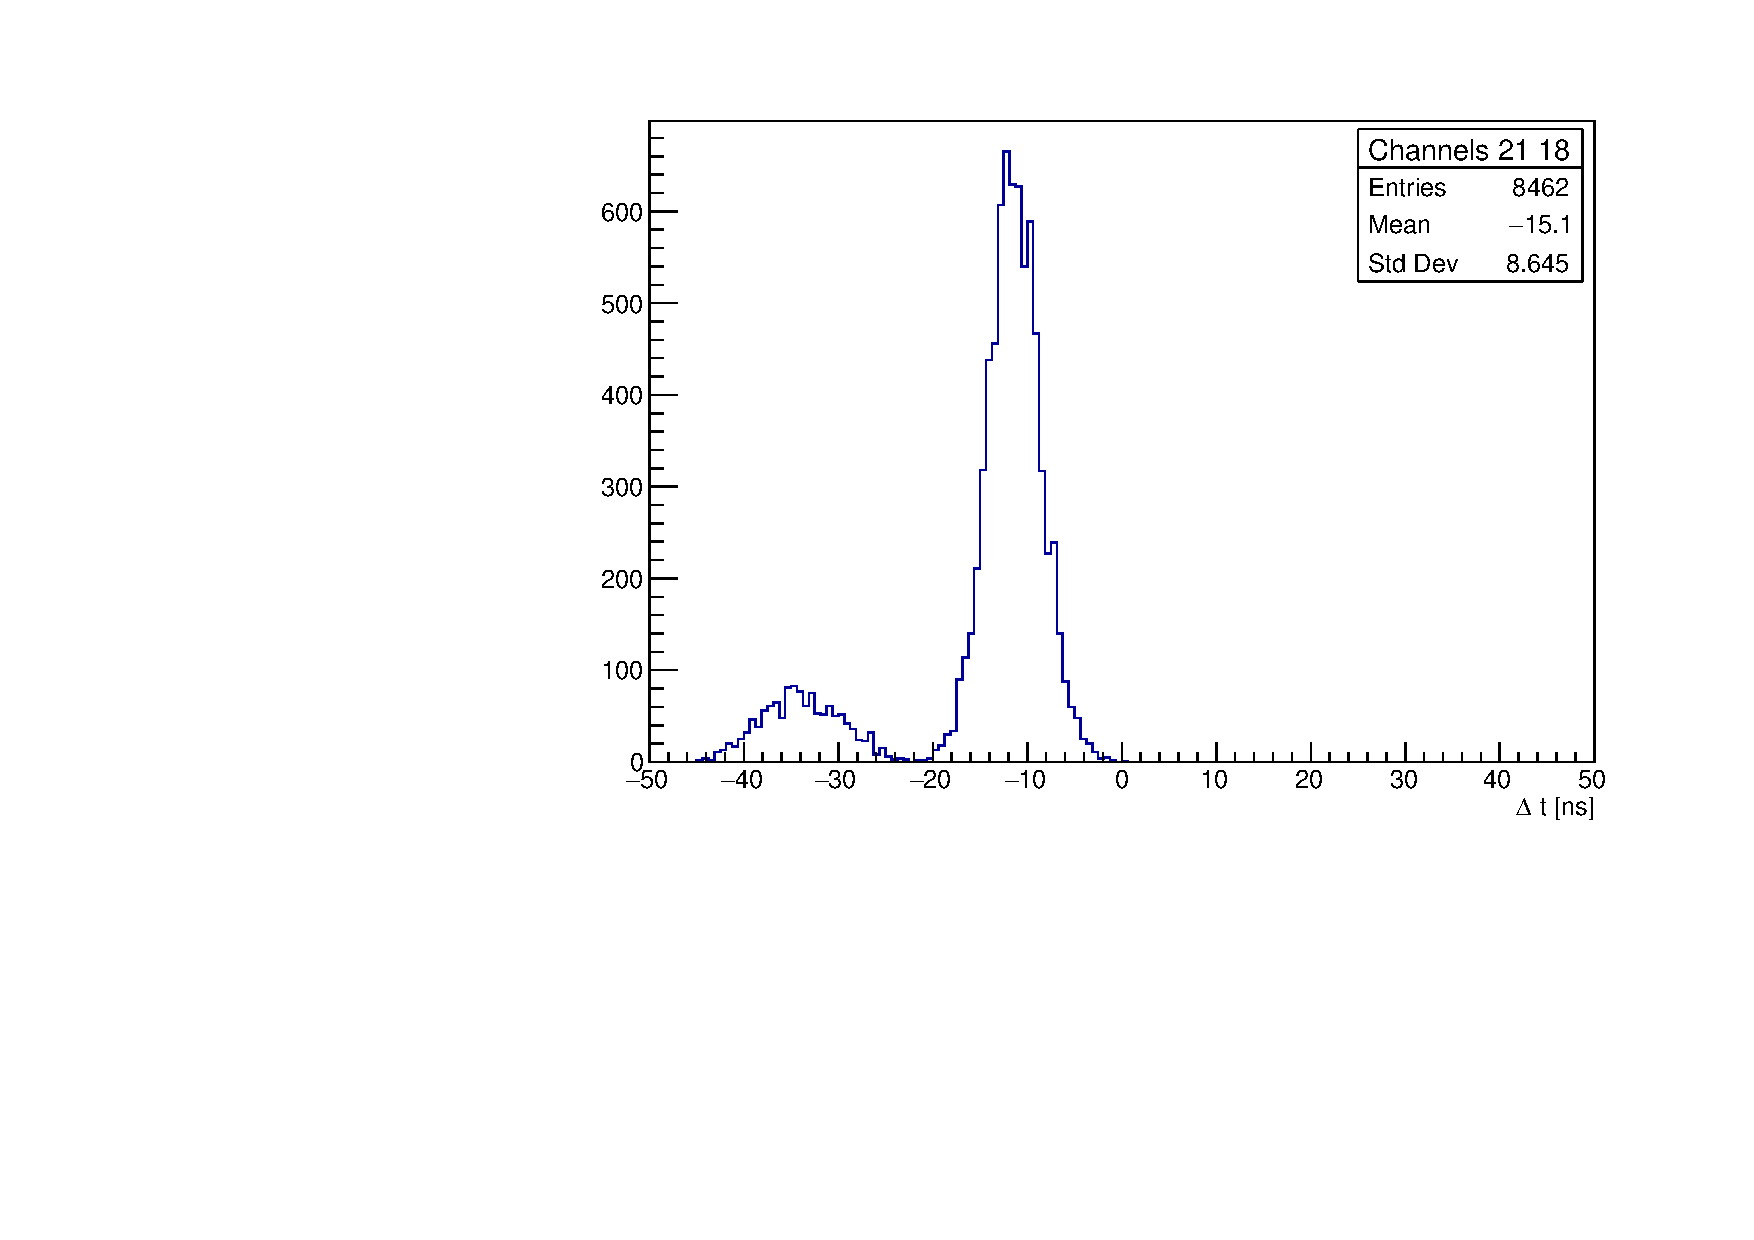
\includegraphics[width=0.49\textwidth]{figures/timingPlots/intraSlice/Channels_21_18.pdf}
    \caption{\label{fig:timeDiffInterSlab} Time differences between each slab and channel 18. 
    The modal values are used to calibrate the inter-slab timing.}
\end{figure}

After applying all previous calibrations the layers are calibrated using beam and cosmic muons hitting all 
four layers, tagged as a muon pulse hitting all four slabs. The mean value of the time difference
relative to the slab closest to the layer is taken as the calibration. Figure~\ref{fig:timeDiffInterLayer}
shows the time difference between the layers and closest slab. The standard deviation ranges from
4.3 to 4.8\unit{ns}.

\begin{figure}
\centering
    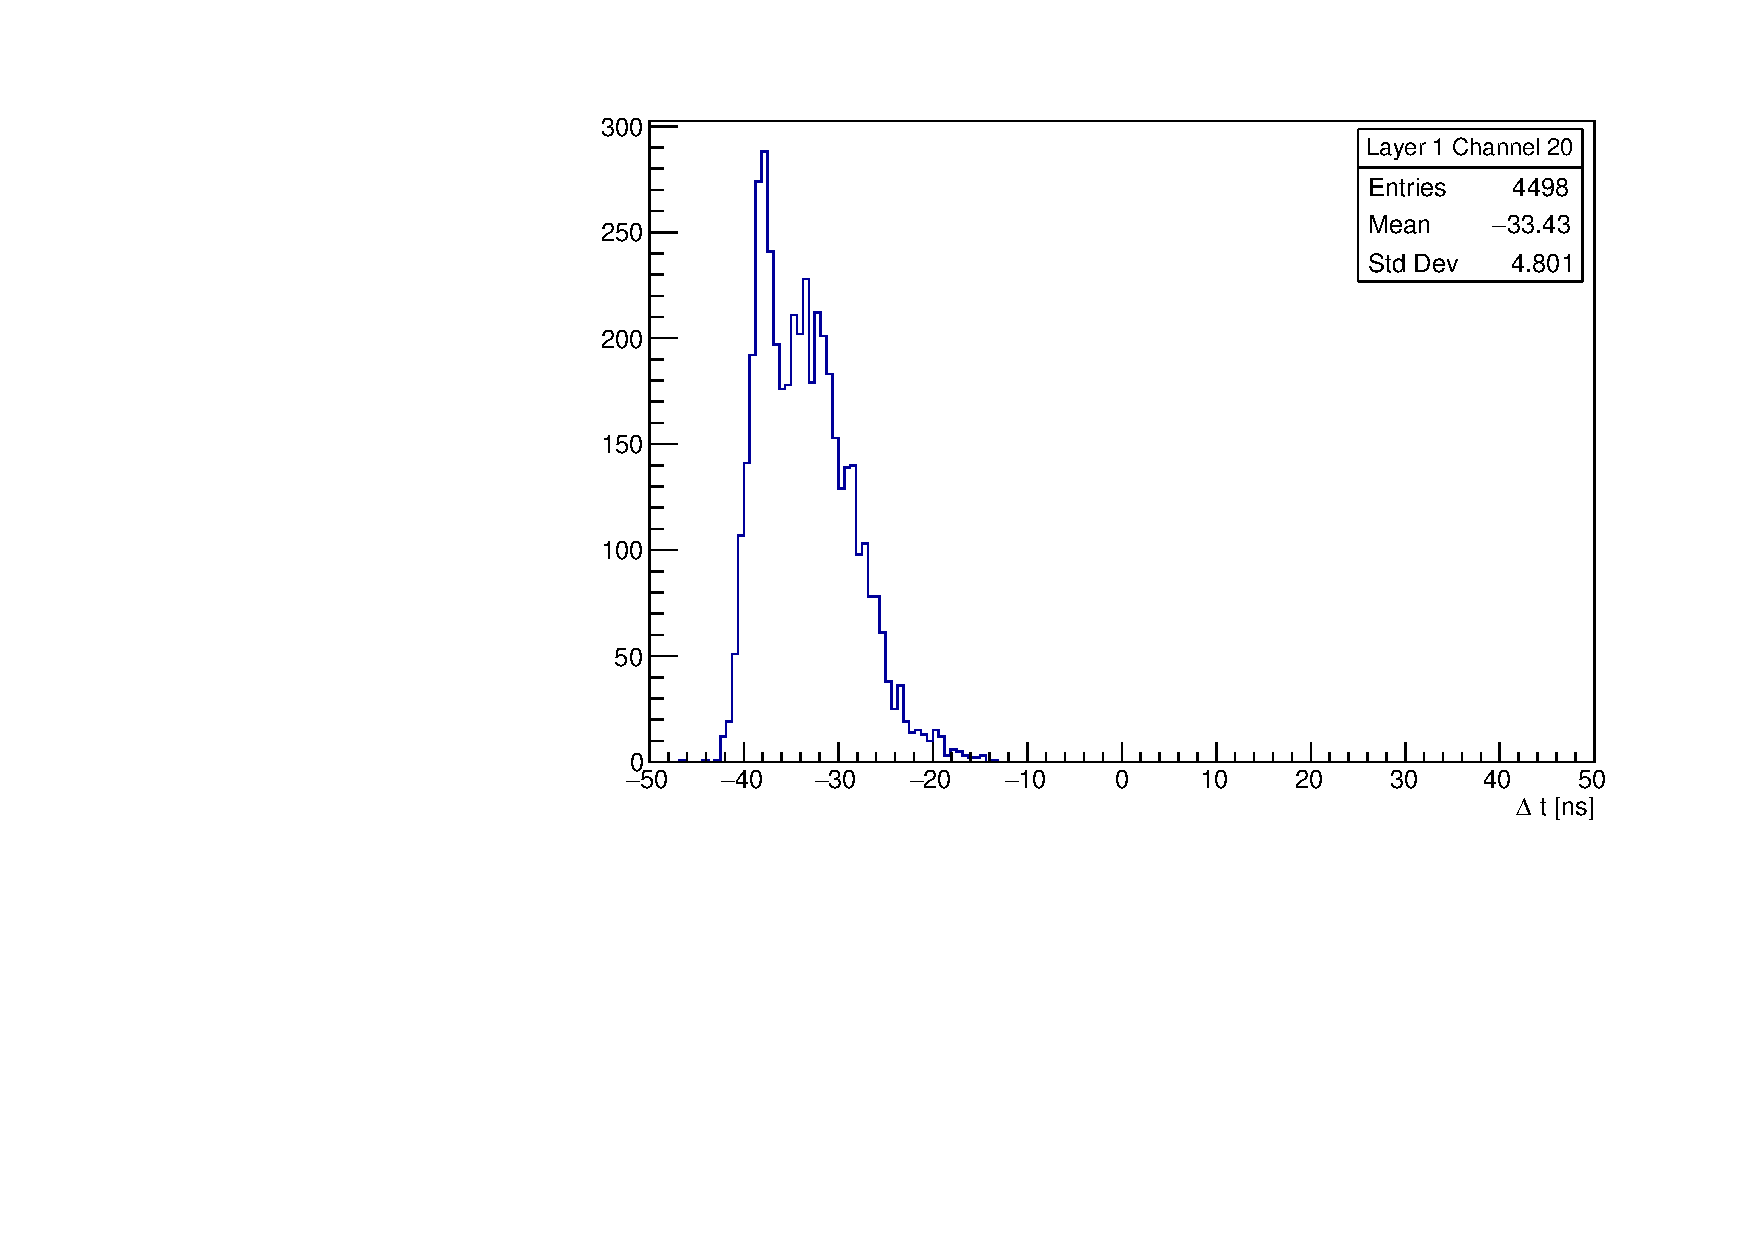
\includegraphics[width=0.49\textwidth]{figures/timingPlots/interLayer/Layer_1_Channel_20.pdf}~
    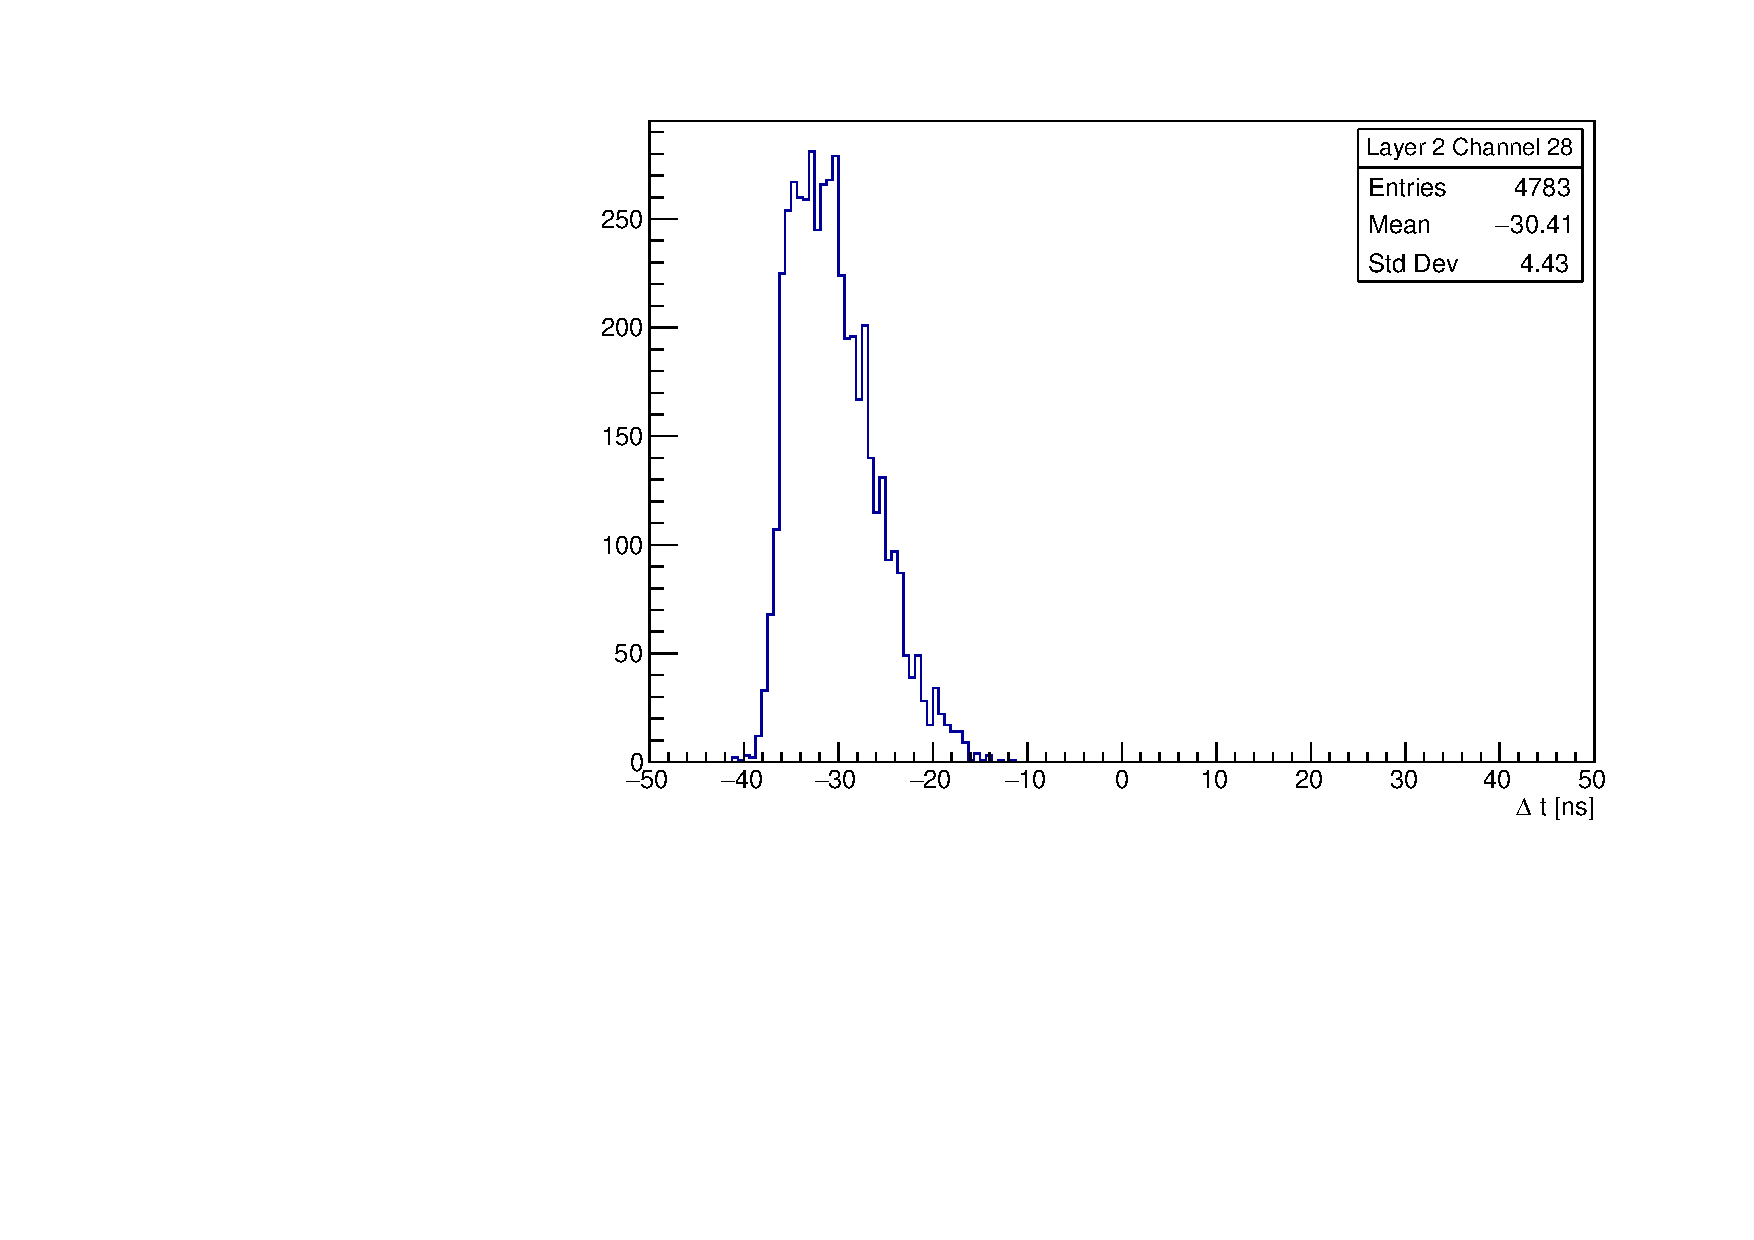
\includegraphics[width=0.49\textwidth]{figures/timingPlots/interLayer/Layer_2_Channel_28.pdf}\\
    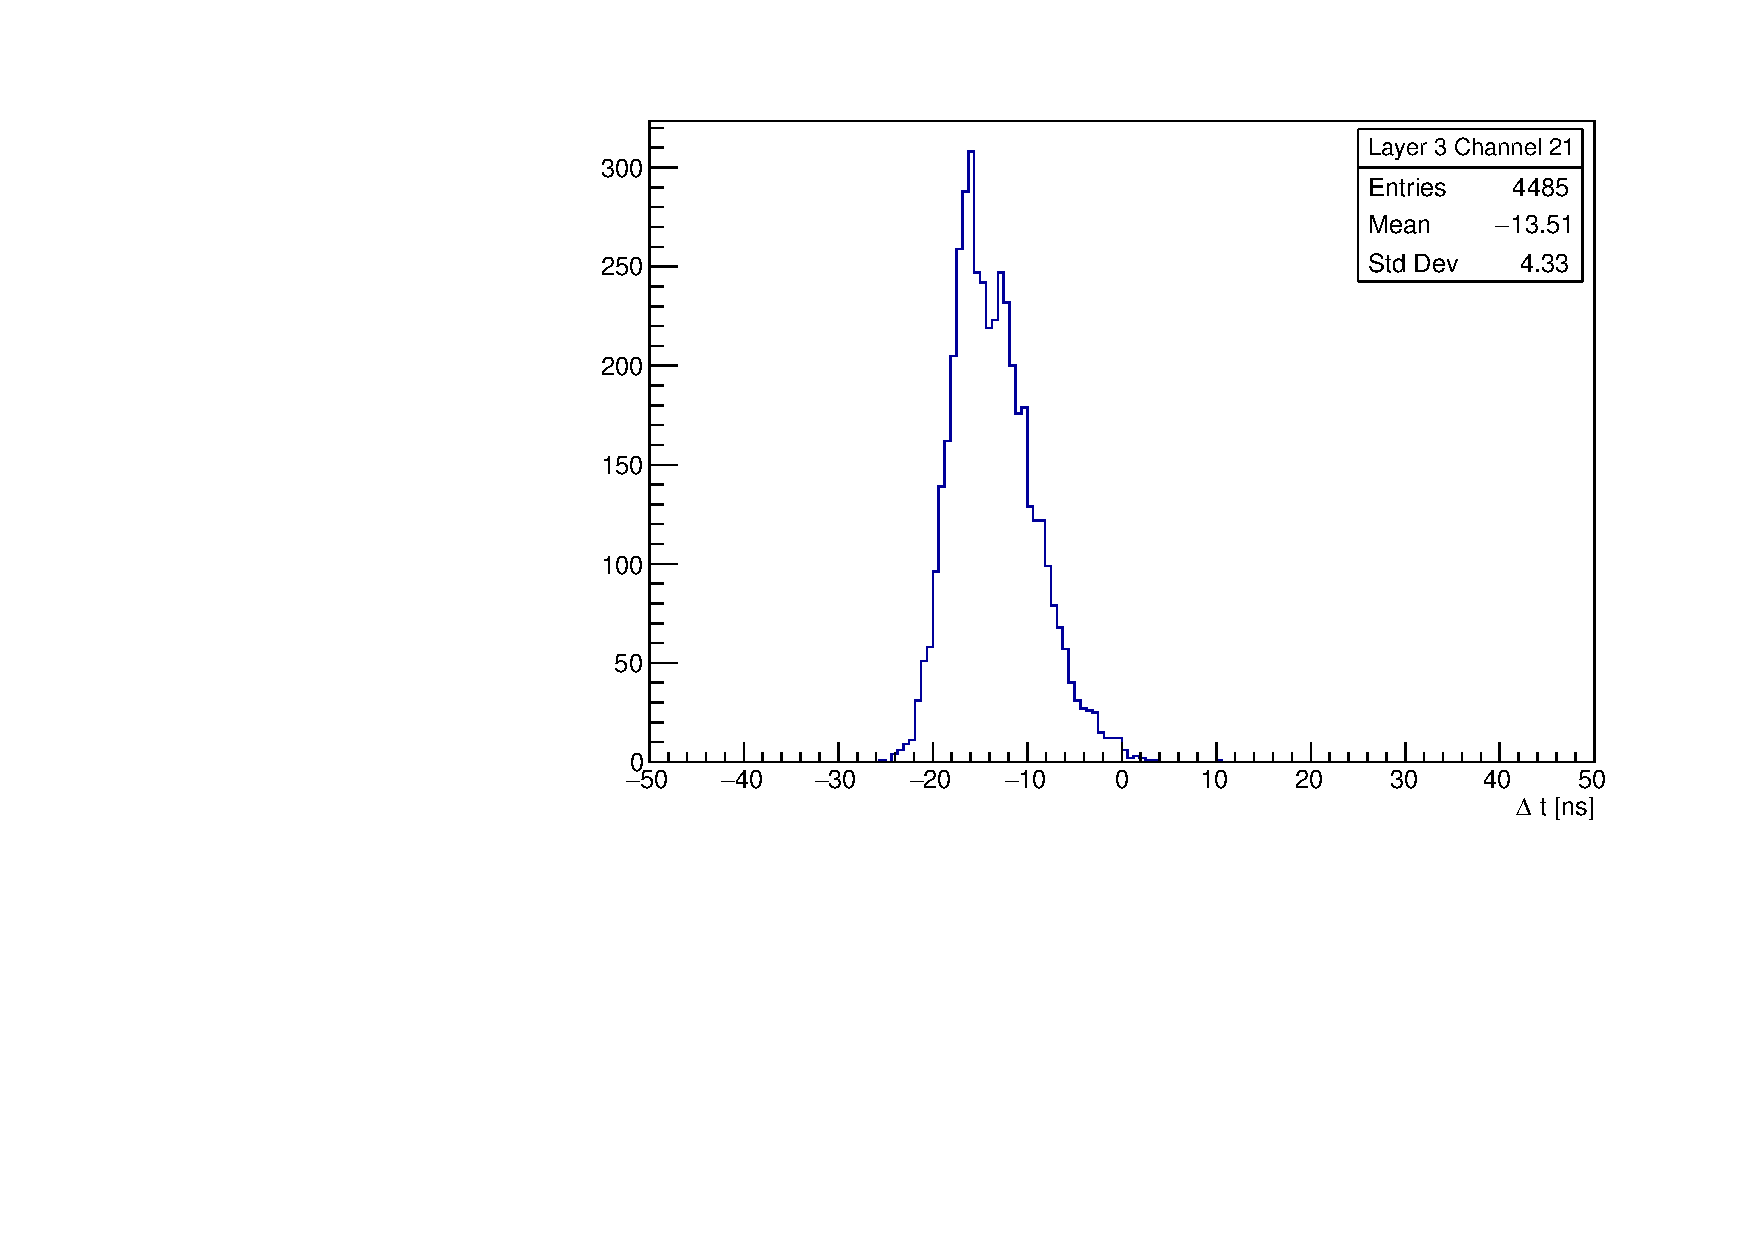
\includegraphics[width=0.49\textwidth]{figures/timingPlots/interLayer/Layer_3_Channel_21.pdf}
    \caption{\label{fig:timeDiffInterLayer} Example time differences between each layer and the closest slab. 
    The mean values are used to calibrate the inter-layer timing.}
\end{figure}

Finally, the panels are calibrated to the layers using cosmic muons tagged as having a muon
pulse in the planel and in the layer closest to the panel. The mean value of the time 
difference relative to the layer is taken as the calibration. Figure~\ref{fig:timeDiffPanelLayer}
shows representative time differences between the panels and the closest layer. The standard deviation ranges
from 5.8 to 8.0\unit{ns}.

\begin{figure}
\centering
    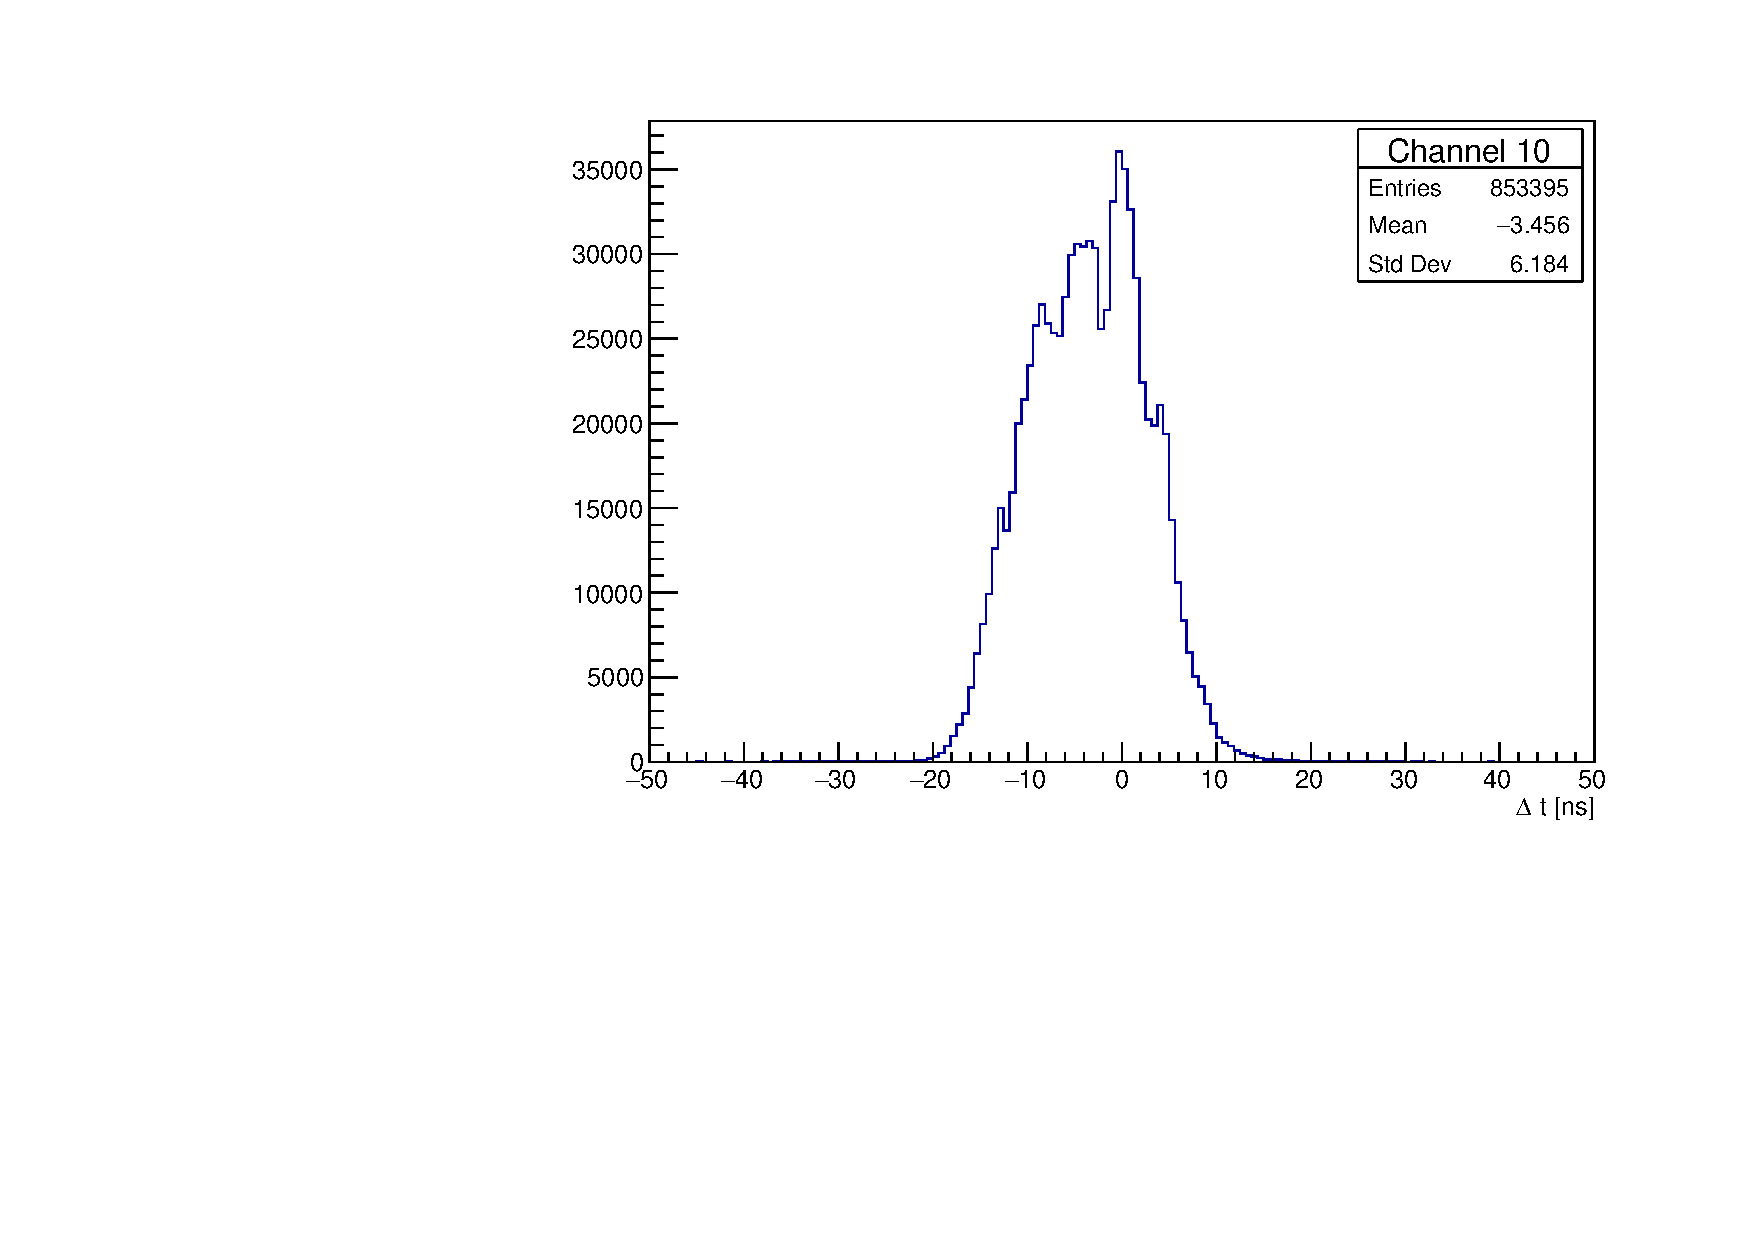
\includegraphics[width=0.49\textwidth]{figures/timingPlots/panels/Channel_10.pdf}~
    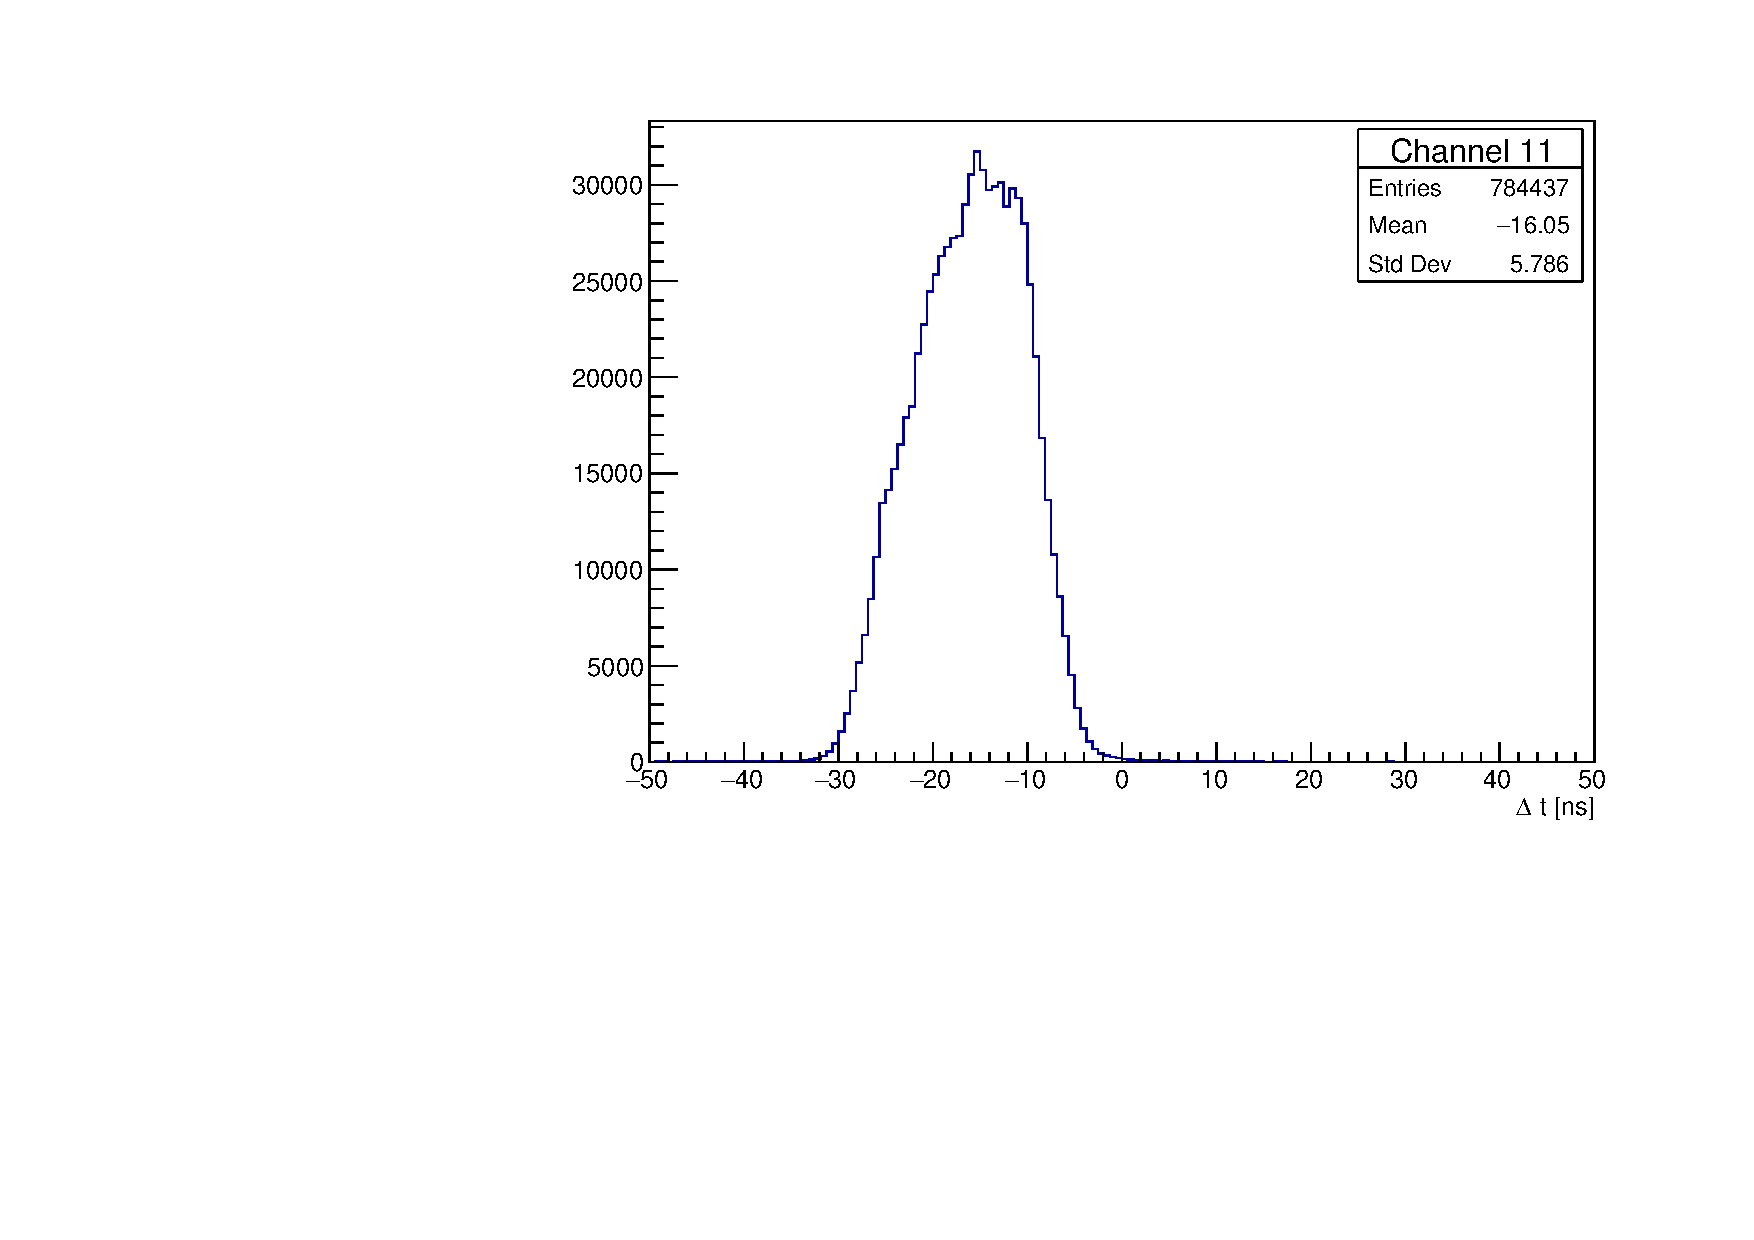
\includegraphics[width=0.49\textwidth]{figures/timingPlots/panels/Channel_11.pdf}\\
    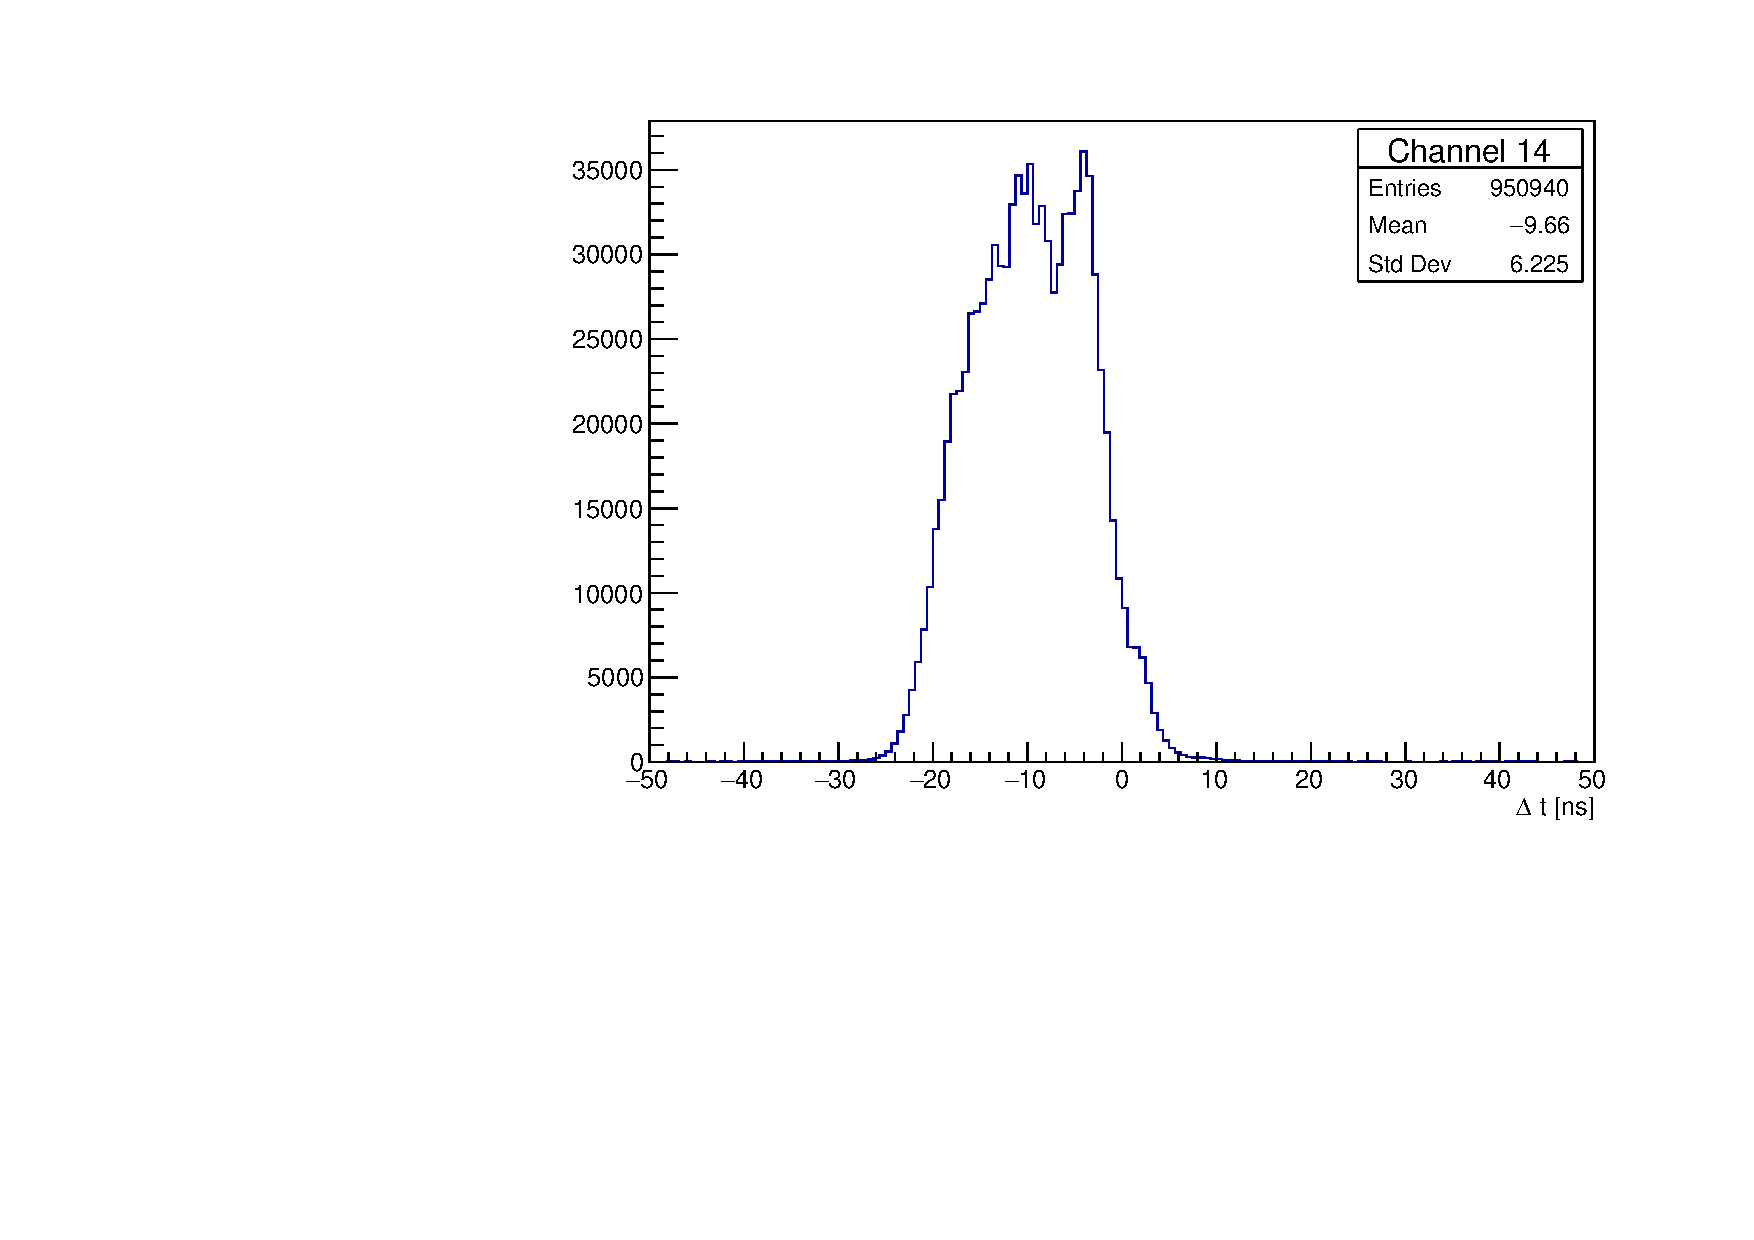
\includegraphics[width=0.49\textwidth]{figures/timingPlots/panels/Channel_14.pdf}~
    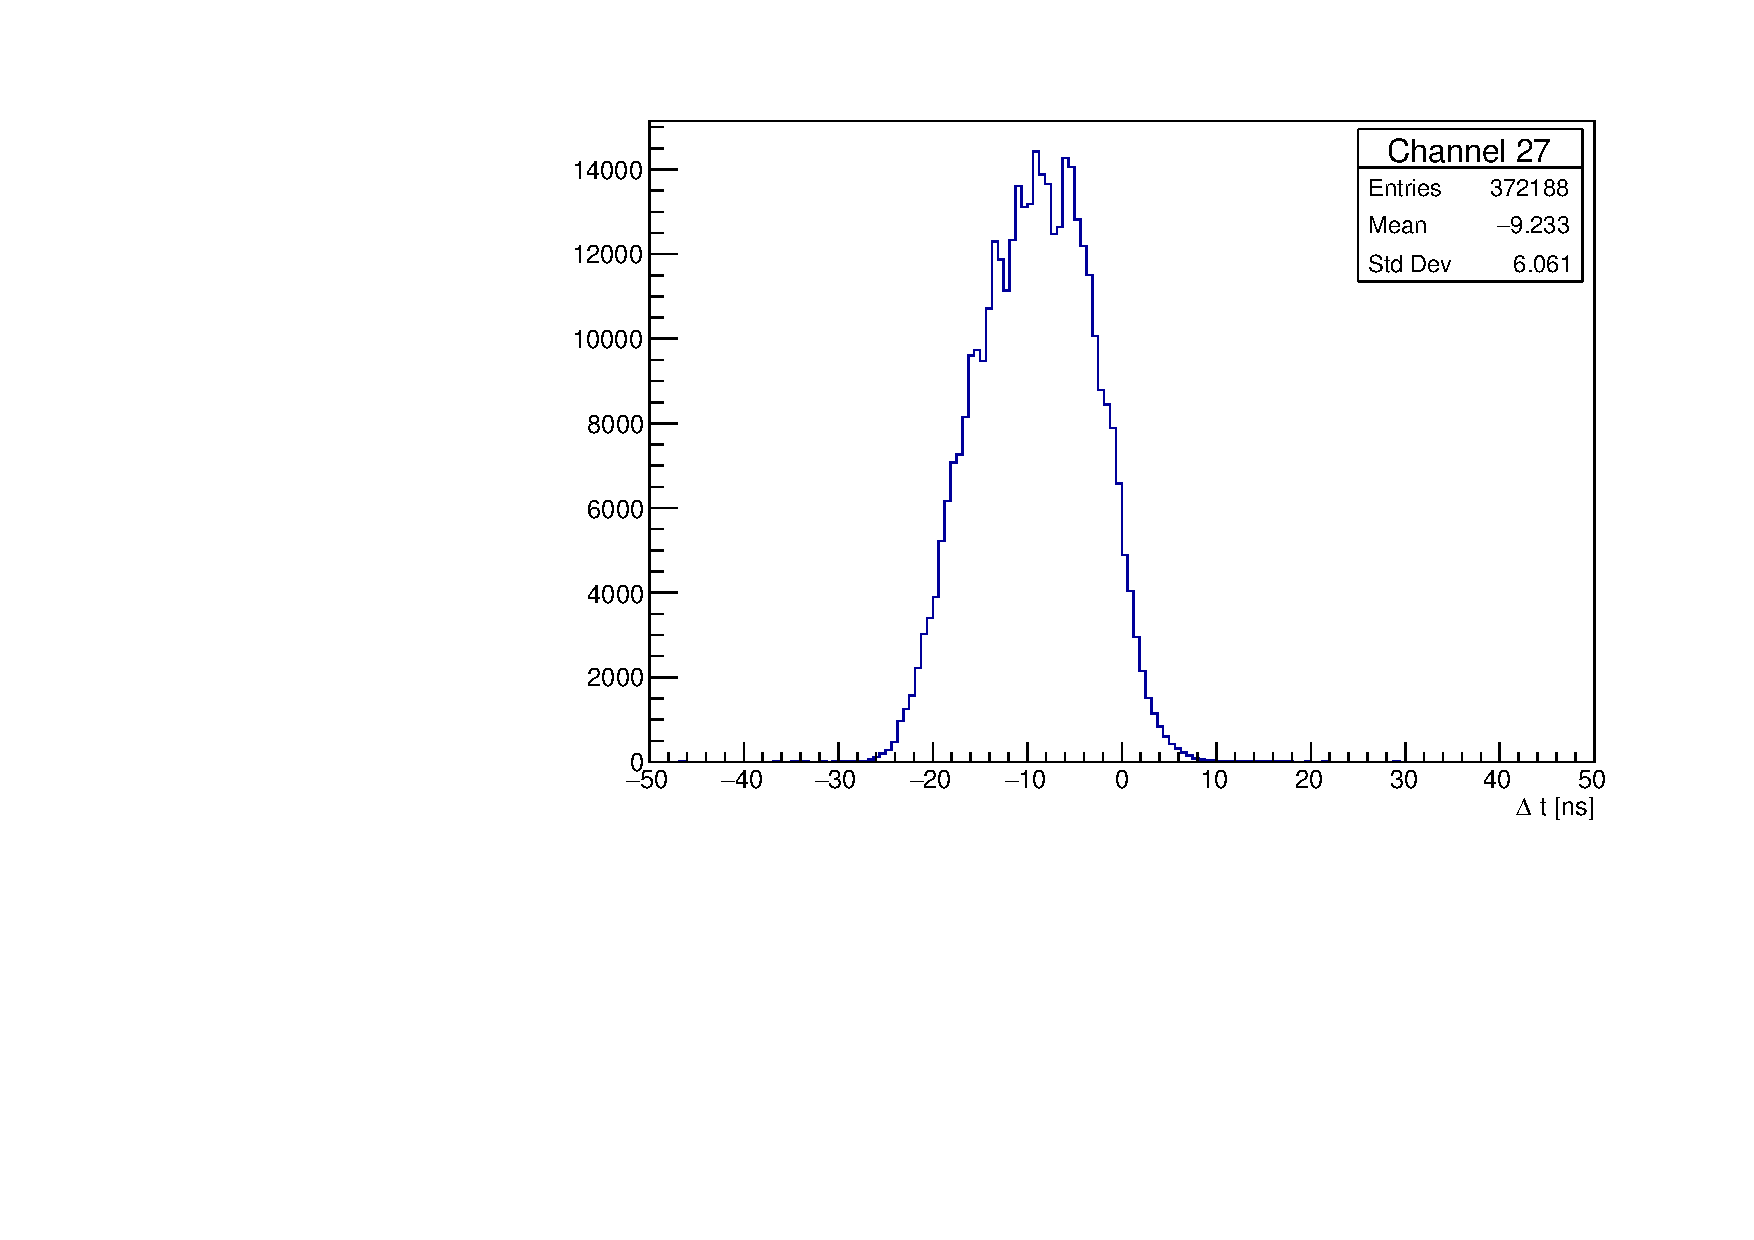
\includegraphics[width=0.49\textwidth]{figures/timingPlots/panels/Channel_27.pdf}
    \caption{\label{fig:timeDiffPanelLayer} Example time differences between panels and the closest layer. 
    The mean values are used to calibrate the panel timing.}
\end{figure}

The calibrations for each channel are summarised in table~\ref{tab:calibrations}. The 
standard deviation in the time difference between layers is $\sim5\unit{ns}$, allowing 
a time window of $15\unit{ns}$ to be defined for signal candidate events, as described in 
Section~\ref{sec:search}.
33.125, 33.125, 13.75, 24.375, 23.75, 35.0, 30.625, 29.375, 24.375, 33.75, 3.75, 16.25, 26.875, 34.375, 9.375, 0.0, 27.5, 30.625, 0.0, 11.25, 7.5, 12.5, 28.125,      20.625, 33.75, 26.875, -3.125, 9.375, 13.75, 0.625, 15.625
\begin{table}[ht!]
    \centering
    \scriptsize
    \topcaption{
	Time calibrations for each channel~\label{tab:calibrations}. The values are added to the raw time to define the calibrated time.
	}
	\begin{tabular}{ll}
	    Channel & Calibration (ns) \\ 
	    \hline
	    0 &  33.125   \\
	    1 &  33.125  \\
	    2 &  13.75   \\ 
	    3 &  24.375  \\
	    4 &  23.75   \\
	    5 &  35.0    \\
	    6 &  30.625  \\
	    7 &  29.375  \\
	    8 &  24.375  \\
	    9 &  33.75   \\
	    10 & 3.75    \\
	    11 & 16.25   \\
	    12 & 26.875  \\  
	    13 & 34.375  \\
	    14 & 9.375   \\
	    15 & --     \\
	    16 & 27.5    \\
	    17 & 30.625  \\
	    18 & 0.0     \\
	    19 & 11.25   \\
	    20 & 7.5     \\
	    21 & 12.5    \\
	    22 & 28.125  \\
	    23 & 20.625  \\
	    24 & 33.75   \\
	    25 & 26.875  \\
	    26 & -3.125  \\
	    27 & 9.375   \\
	    28 & 13.75   \\
	    29 & 0.625   \\
	    30 & 15.625  \\
	    31 & 10.625     \\ 
	\end{tabular}
\end{table}

\section{Alignment}

The alignment of the demonstrator is tested using muons originating from the proton-proton collisions 
at CMS. Figure~\ref{fig:occ2d} shows the dependence of the total number of particles identified as having a muon pulse
in all four slabs on the luminosity of the LHC fill measured by CMS. There is a clear linear dependence with
a muon rate of $0.19/\pbinv$ measured in data, which agrees with the expected value from simulation
of a muon rate of $0.22/\pbinv$. This provides confidence the demonstrator is correctly aligned 
with the CMS interaction point.

\begin{figure}[ht!]
    \centering
    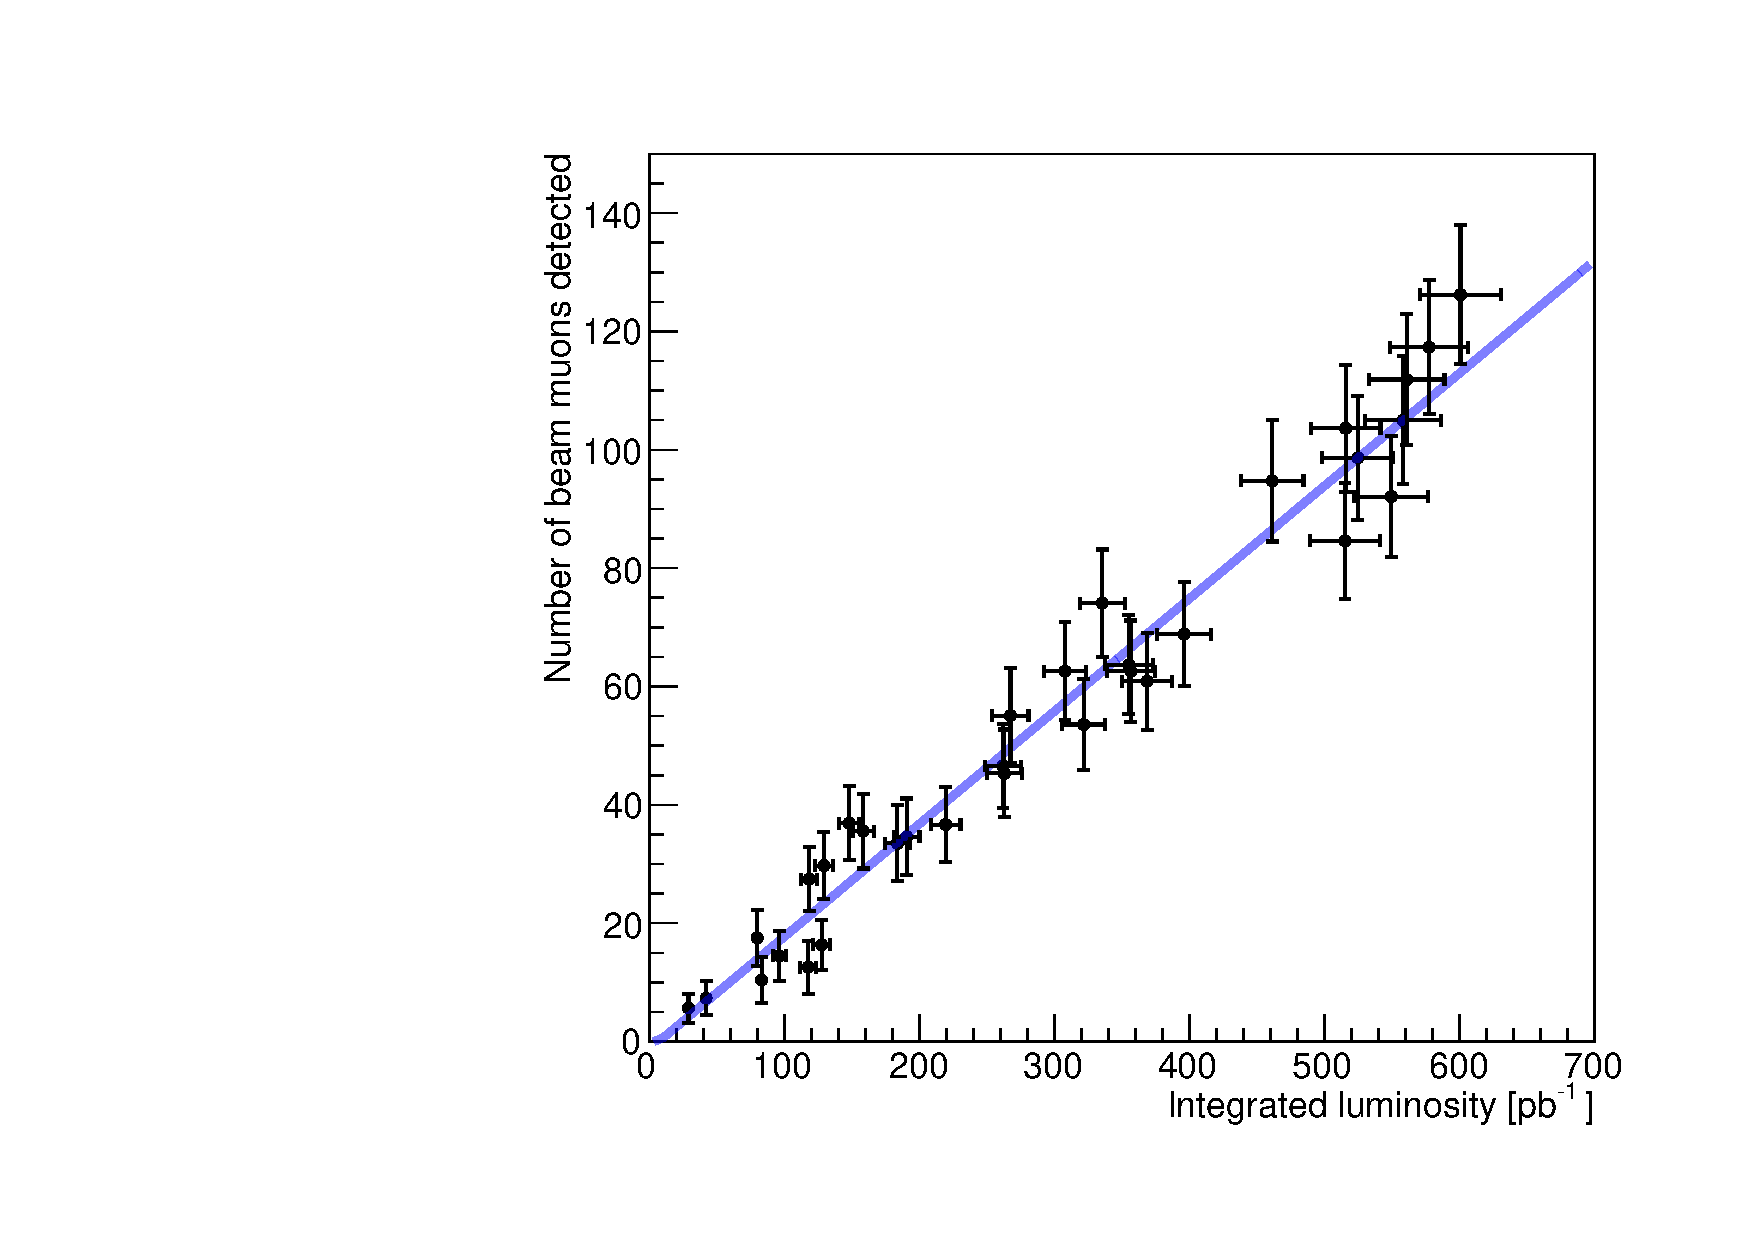
\includegraphics[width=0.6\textwidth]{figures/occ2d}
    \caption{\label{fig:occ2d} The occupancy of the milliQan demonstrator as a function of luminosity}
\end{figure}

The time difference between the slabs closest and furthest from the beam after the 
calibration described in Section~\ref{sec:timeCalibration} also provides confirmation
that the pulse timing can be used to accurately identify muons originating from the beam. 
Figure~\ref{fig:timeDiff} shows well separated peaks from beam and cosmic muons with a time difference
consistent with that expected from the geometrical distance between the slabs 
($2\times3.6/0.3 = 22\unit{ns}$).

\begin{figure}[ht!]
    \centering
    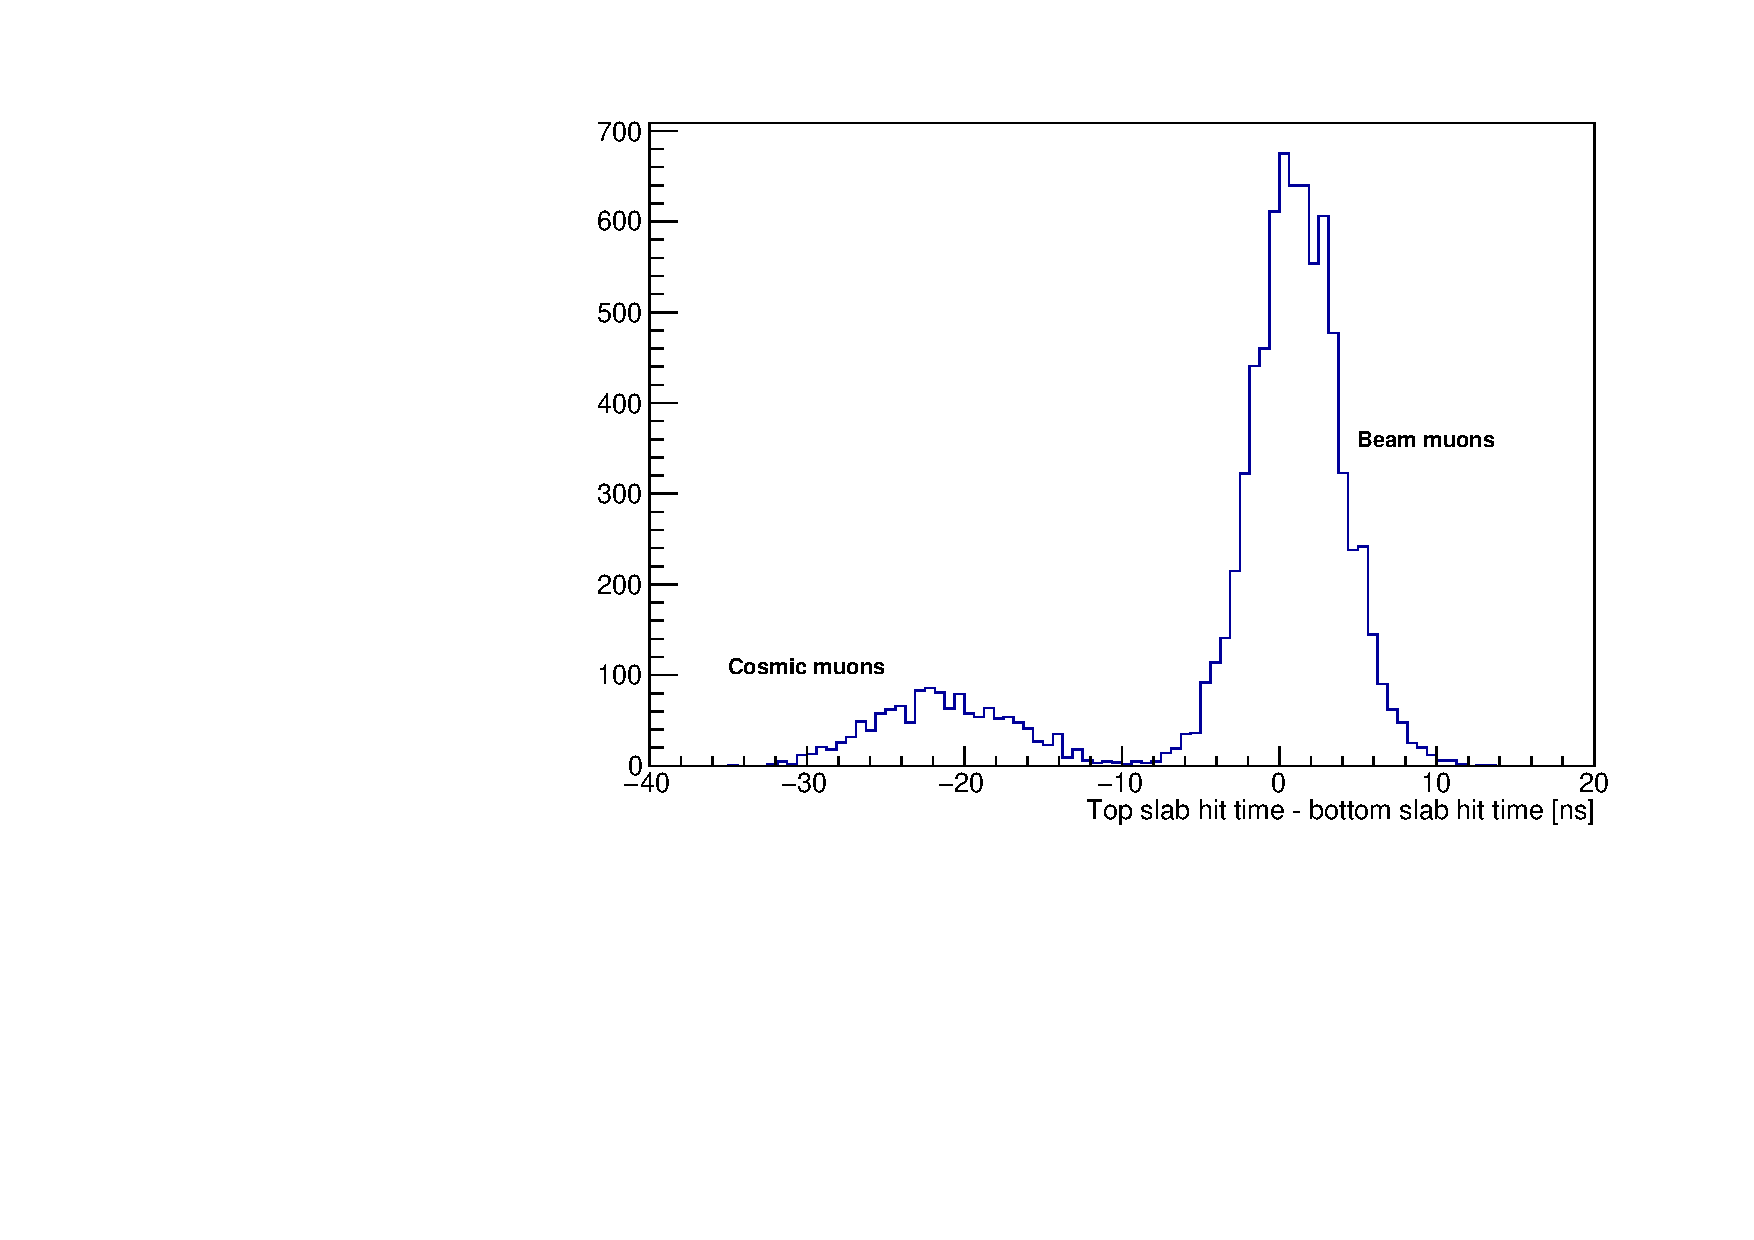
\includegraphics[width=0.6\textwidth]{figures/timeDiffSlabs}
    \caption{\label{fig:timeDiff} Time difference between the slabs furthest and closest to the CMS IP (channels 21 and 18 respectively).}
\end{figure}

\section{Search design}
\label{sec:search}

Rejection of known backgrounds through signal selections

\section{Background determination}

Measurements of residual backgrounds

\section{Interpretation}

Signal efficiencies from injection tests and prototype interpretations

\section{Summary}

Conclusions

\end{document}
